% A LaTeX template for MSc Thesis submissions to 
% Politecnico di Milano (PoliMi) - School of Industrial and Information Engineering
%
% S. Bonetti, A. Gruttadauria, G. Mescolini, A. Zingaro
% e-mail: template-tesi-ingind@polimi.it
%
% Last Revision: October 2021
%
% Copyright 2021 Politecnico di Milano, Italy. NC-BY

\documentclass{Configuration_Files/PoliMi3i_thesis}

%------------------------------------------------------------------------------
%	REQUIRED PACKAGES AND  CONFIGURATIONS
%------------------------------------------------------------------------------

% CONFIGURATIONS
\usepackage{parskip} % For paragraph layout
\usepackage{setspace} % For using single or double spacing
\usepackage{emptypage} % To insert empty pages
\usepackage{multicol} % To write in multiple columns (executive summary)
\setlength\columnsep{15pt} % Column separation in executive summary
\setlength\parindent{0pt} % Indentation
\raggedbottom  

% PACKAGES FOR TITLES
\usepackage{titlesec}
% \titlespacing{\section}{left spacing}{before spacing}{after spacing}
\titlespacing{\section}{0pt}{3.3ex}{2ex}
\titlespacing{\subsection}{0pt}{3.3ex}{1.65ex}
\titlespacing{\subsubsection}{0pt}{3.3ex}{1ex}
\usepackage{color}

% PACKAGES FOR LANGUAGE AND FONT
\usepackage[english]{babel} % The document is in English  
\usepackage[utf8]{inputenc} % UTF8 encoding
\usepackage[T1]{fontenc} % Font encoding
\usepackage[11pt]{moresize} % Big fonts
\usepackage{ragged2e}

% PACKAGES FOR IMAGES
\usepackage{graphicx}
\usepackage{transparent} % Enables transparent images
\usepackage{eso-pic} % For the background picture on the title page
\usepackage{subfig} % Numbered and caption subfigures using \subfloat.
\usepackage{tikz} % A package for high-quality hand-made figures.
\usetikzlibrary{}
\graphicspath{{./Images/}} % Directory of the images
\usepackage{caption} % Coloured captions
\usepackage{xcolor} % Coloured captions
\usepackage{amsthm,thmtools,xcolor} % Coloured "Theorem"
\usepackage{float}
\usepackage[outdir=./Images]{epstopdf} % Finding and converting eps images
\usepackage{wrapfig}


% STANDARD MATH PACKAGES
\usepackage{amsmath}
\usepackage{amsthm}
\usepackage{amssymb}
\usepackage{amsfonts}
\usepackage{bm}
\usepackage[overload]{empheq} % For braced-style systems of equations.
\usepackage{fix-cm} % To override original LaTeX restrictions on sizes

% PACKAGES FOR TABLES
\usepackage{tabularx}
\usepackage{longtable} % Tables that can span several pages
\usepackage{colortbl}
\usepackage{multirow}
\usepackage{array}

% PACKAGES FOR ALGORITHMS (PSEUDO-CODE)
\usepackage{algorithm}
\usepackage{algorithmic}

% PACKAGES FOR REFERENCES & BIBLIOGRAPHY
\usepackage[colorlinks=true,linkcolor=black,anchorcolor=black,citecolor=black,filecolor=black,menucolor=black,runcolor=black,urlcolor=black]{hyperref} % Adds clickable links at references
\usepackage{cleveref}
\usepackage[square, numbers, sort&compress]{natbib} % Square brackets, citing references with numbers, citations sorted by appearance in the text and compressed
\bibliographystyle{abbrvnat} % You may use a different style adapted to your field

% OTHER PACKAGES
\usepackage{pdfpages} % To include a pdf file
\usepackage{afterpage}
\usepackage{lipsum} % DUMMY PACKAGE
\usepackage{fancyhdr} % For the headers
\fancyhf{}

% Input of configuration file. Do not change config.tex file unless you really know what you are doing. 
% Define blue color typical of polimi
\definecolor{bluepoli}{cmyk}{0.4,0.1,0,0.4}

% Custom theorem environments
\declaretheoremstyle[
  headfont=\color{bluepoli}\normalfont\bfseries,
  bodyfont=\color{black}\normalfont\itshape,
]{colored}

% Set-up caption colors
\captionsetup[figure]{labelfont={color=bluepoli}} % Set colour of the captions
\captionsetup[table]{labelfont={color=bluepoli}} % Set colour of the captions
\captionsetup[algorithm]{labelfont={color=bluepoli}} % Set colour of the captions

\theoremstyle{colored}
\newtheorem{theorem}{Theorem}[chapter]
\newtheorem{proposition}{Proposition}[chapter]

% Enhances the features of the standard "table" and "tabular" environments.
\newcommand\T{\rule{0pt}{2.6ex}}
\newcommand\B{\rule[-1.2ex]{0pt}{0pt}}

% Pseudo-code algorithm descriptions.
\newcounter{algsubstate}
\renewcommand{\thealgsubstate}{\alph{algsubstate}}
\newenvironment{algsubstates}
  {\setcounter{algsubstate}{0}%
   \renewcommand{\STATE}{%
     \stepcounter{algsubstate}%
     \Statex {\small\thealgsubstate:}\space}}
  {}

% New font size
\newcommand\numfontsize{\@setfontsize\Huge{200}{60}}

% Title format: chapter
\titleformat{\chapter}[hang]{
\fontsize{50}{20}\selectfont\bfseries\filright}{\textcolor{bluepoli} \thechapter\hsp\hspace{2mm}\textcolor{bluepoli}{|   }\hsp}{0pt}{\huge\bfseries \textcolor{bluepoli}
}

% Title format: section
\titleformat{\section}
{\color{bluepoli}\normalfont\Large\bfseries}
{\color{bluepoli}\thesection.}{1em}{}

% Title format: subsection
\titleformat{\subsection}
{\color{bluepoli}\normalfont\large\bfseries}
{\color{bluepoli}\thesubsection.}{1em}{}

% Title format: subsubsection
\titleformat{\subsubsection}
{\color{bluepoli}\normalfont\large\bfseries}
{\color{bluepoli}\thesubsubsection.}{1em}{}

% Shortening for setting no horizontal-spacing
\newcommand{\hsp}{\hspace{0pt}}

\makeatletter
% Renewcommand: cleardoublepage including the background pic
\renewcommand*\cleardoublepage{%
  \clearpage\if@twoside\ifodd\c@page\else
  \null
  \AddToShipoutPicture*{\BackgroundPic}
  \thispagestyle{empty}%
  \newpage
  \if@twocolumn\hbox{}\newpage\fi\fi\fi}
\makeatother

%For correctly numbering algorithms
\numberwithin{algorithm}{chapter}

%----------------------------------------------------------------------------
%	NEW COMMANDS DEFINED
%----------------------------------------------------------------------------

% EXAMPLES OF NEW COMMANDS
\newcommand{\bea}{\begin{eqnarray}} % Shortcut for equation arrays
\newcommand{\eea}{\end{eqnarray}}
\newcommand{\e}[1]{\times 10^{#1}}  % Powers of 10 notation

%----------------------------------------------------------------------------
%	ADD YOUR PACKAGES (be careful of package interaction)
%----------------------------------------------------------------------------

%----------------------------------------------------------------------------
%	ADD YOUR DEFINITIONS AND COMMANDS (be careful of existing commands)
%----------------------------------------------------------------------------

%----------------------------------------------------------------------------
%	BEGIN OF YOUR DOCUMENT
%----------------------------------------------------------------------------

\begin{document}

\fancypagestyle{plain}{%
\fancyhf{} % Clear all header and footer fields
\fancyhead[RO,RE]{\thepage} %RO=right odd, RE=right even
\renewcommand{\headrulewidth}{0pt}
\renewcommand{\footrulewidth}{0pt}}

%----------------------------------------------------------------------------
%	TITLE PAGE
%----------------------------------------------------------------------------

\pagestyle{empty} % No page numbers
\frontmatter % Use roman page numbering style (i, ii, iii, iv...) for the preamble pages

\puttitle{
	title=Procedural Decoration of DOOM Levels with Generative Adversarial Networks, % Title of the thesis
	name=Akash Aloysius James, % Author Name and Surname
	course=Ingegneria Informatica, % Study Programme (in Italian)
	ID  = 10687690,  % Student ID number (numero di matricola)
	advisor= Daniele Loiacono, % Supervisor name
	coadvisor={Pierluca Lanzi}, % Co-Supervisor name, remove this line if there is none
	academicyear={2022-23},  % Academic Year
} % These info will be put into your Title page 

%----------------------------------------------------------------------------
%	PREAMBLE PAGES: ABSTRACT (inglese), EXECUTIVE SUMMARY
%----------------------------------------------------------------------------
\startpreamble
\setcounter{page}{1} % Set page counter to 1

% ABSTRACT IN ENGLISH
\chapter*{Abstract} 
This study examines how to automate the process of populating procedurally 
generated levels using Conditional Adversarial Networks. The goal is to spawn 
game objects in a manner that functionally mimics the characteristics of those present 
in human designed levels without the need to explicitly define an exhaustive set of
rules to govern the system. It is meant to enhance the level building process by 
upgrading the process of including content within the generated DOOM levels. The initial 
objective is to produce a coherent topology, accompanied by a suitable availability and 
positioning of game objects with respect to the level layout. This requires addressing 
complications that impede consistent representation and generation from the previous 
design. Then the modifications are compiled together to fashion a generative system 
that can construct the minimum sufficient subset of features used to design a unique level. 
Finally, a comparison is made between the modified system and the prior architecture to 
highlight the improvements it provides in regard to what was previously feasible.
These samples are evaluated in a manner that contrasts the differences present 
among them and those available in the repository. The outcome of these experiments 
should prove a degree of competence in the system’s ability for level design and act 
as a practical alternative for the implementation of procedural content generation for 
games to come.
\\
\\

% ABSTRACT IN ITALIAN
\chapter*{Abstract in lingua italiana}
Questa tesi esamina come automatizzare il popolamento di livelli generati proceduralmente utilizzando delle Conditional Adversarial Networks. L'obiettivo è generare oggetti di gioco in modo tale da imitare dal punto di vista funzionale  le caratteristiche di quelli presenti nei livelli progettati dall'uomo, senza la necessità di definire esplicitamente un insieme esaustivo di regole a questo scopo. L'obbiettivo è migliorare il processo di creazione dei livelli, potenziando il processo di inserimento di contenuti all'interno dei livelli generati di DOOM. L'obiettivo iniziale è produrre una topologia coerente, accompagnata da una disponibilità e posizionamento adeguati degli oggetti di gioco rispetto alla struttura del livello. Ciò richiede di affrontare complicazioni che ostacolano la rappresentazione e la generazione di contenuti coerenti a partire dal design originale. Successivamente, le componenti progettate vengono combinate per creare un sistema generativo in grado di costruire il sottoinsieme minimo sufficiente di caratteristiche utilizzate per progettare un livello unico. Infine, viene effettuato un confronto tra il sistema modificato e i precedenti lavori per evidenziare i miglioramenti che offre rispetto a quanto era precedentemente possibile. I livelli generati sono stati valutati in modo da evidenziare le differenze con i livelli disponibili nel repository. Il risultato di questa analisi sperimentale consente di dimostrare un certo grado di competenza del sistema nella progettazione dei livelli, offrendo un'alternativa pratica per l'implementazione della generazione procedurale di contenuti per i giochi futuri.
\\
\\


%----------------------------------------------------------------------------
%	LIST OF CONTENTS/FIGURES/TABLES/SYMBOLS
%----------------------------------------------------------------------------

% TABLE OF CONTENTS
\thispagestyle{empty}
\tableofcontents % Table of contents 
\thispagestyle{empty}
\cleardoublepage

%-------------------------------------------------------------------------
%	THESIS MAIN TEXT
%-------------------------------------------------------------------------
% In the main text of your thesis you can write the chapters in two different ways:
%
%(1) As presented in this template you can write:
%    \chapter{Title of the chapter}
%    *body of the chapter*
%
%(2) You can write your chapter in a separated .tex file and then include it in the main file with the following command:
%    \chapter{Title of the chapter}
%    \input{chapter_file.tex}
%
% Especially for long thesis, we recommend you the second option.

\addtocontents{toc}{\vspace{2em}} % Add a gap in the Contents, for aesthetics
\mainmatter % Begin numeric (1,2,3...) page numbering

% --------------------------------------------------------------------------
% NUMBERED CHAPTERS % Regular chapters following
% --------------------------------------------------------------------------
\chapter{Introduction}
\label{ch:introduction}%
% The \label{...}% enables to remove the small indentation that is generated, always leave the % symbol.

The perceived value of video games as a recreational activity is deeply rooted in the 
duration and intensity that they manage to keep players engaged. A few decades 
ago, as fewer games were released within any given period, developers would often 
try to prolong gameplay to validate the costs. This was achieved with irregular 
difficulty spikes and concealing information which would cause players to take several 
months to complete when coupled with the absence of the ability to retrieve 
one’s progress. In comparison, despite numerous technological advances and man hours 
put into creating vast maps and longer stories, games today can be completed much 
sooner. This is partly due to adjustable difficulty, save points and widely available 
walkthroughs, thereby providing a shorter gameplay at a significant cost to the consumer. 
The novelty also quickly wears off on repeated playthroughs and feels monotonous, 
especially when there are limited to no variations in gameplay, affecting a game’s 
ability to retain players engagement over longer duration.

Replayability is the player’s desire to continue playing a game even after 
experiencing the content, either to optimize one’s skill or to explore for its hidden 
content. It is beneficial as this kind of dedication arises from player satisfaction and 
has been shown to improve brand loyalty \cite{TiF11}, yet many studios struggle to meet these 
expectations. This is usually attributed to the difficulty in maintaining player 
engagement over repeated sessions as it is critical that players don't know how every 
aspect of any level has been laid out. Some of the ways used to tackle this are by 
bringing in competitive aspects such as leaderboards or regular introduction of new 
content through updates which is heavily use of by many Massive Multiplayer Online 
Role Playing Games (MMORPGs) in order to maintain an active player base. The focus of this 
thesis is to address this problem by avoiding the monotony of traversing the same level through 
variations introduced in the level design.
\newpage

\section{Background}
\label{sec:background}
An approach that has long been resorted to combat repetitiveness in replay is 
procedural generation. Early adopters of the technology include games such as 
Rogue \cite{MiT80} with its procedurally generated dungeon and the trading game Elite \cite{DaB84}, 
where each of its planets had randomly determined compositions. The former has 
spawned its own genre called ‘roguelike’ that initially used a similar tile-based 
procedural system. The notion of randomly generating levels solely utilizing existing 
assets at each instance appears more and more appealing as an alternative to 
constructing complex game worlds as it avoids excessive dependence on content 
design. This is especially true for newer games as there is greater demand for more 
content while maintaining graphics at a high fidelity. AAA titles such as Civilization 
\cite{MiP96} use random seeds in complex models to create different worlds for players to 
traverse and explore based on variation of terrain and resource placements while No Man’s Sky 
\cite{HaG16} progressively generates entire galaxies, including stars and planets with flora, 
fauna, and even alien encounters upon discovery.

\section{Problem}
\label{sec:problem}
While procedural generation is not new, it is an exhaustive process which requires 
consideration of minute details when building the system. AI has been developed for 
games, such as playing Infinite Super Mario levels \cite{KaS12} but have been less proficient 
when it comes to replicating creative tasks such as level design as the sample space natively 
adds a greater degree of complexity to the problem. In an attempt to avoid these 
pitfalls and consume vast amounts of resources for creating multiple levels, 
exploring deep learning seems to be a favorable course of action. There is a detailed 
method that is capable of generating DOOM level given certain input criteria 
through the use of conditional Wasserstein Generative Adversarial Networks with Gradient Penalty 
(WGAN-GP) \cite{MaA17} and the help of a large 
repository of custom-made levels created by the community to train the model. 
While the level layout generated by this model has proven adequate for a  
First Person Shooter (FPS), it is unable to place appropriate game objects into the level layout. 
This is because it is plagued with disproportionate generation of game object among the present 
categories and is biased with their placements as it clumps them together in certain sections of the 
level. This results in levels being unevenly saturated and predisposed towards certain types of 
game objects which hampers the level’s ability to properly captivate the player’s 
interest.

\section{Goals}
To improve the DOOM level generator by splitting the problems of planning the level 
layout and populating it with game objects through the introduction of a hybrid 
Generative Adversarial Network (GAN) architecture. This requires a repository of DOOM 
levels that need to be parsed into minimal structures that accurately represent the problematic 
features. With the feature maps serving as the examples to learn from, the hybrid architecture needs to be 
trained on the different aspects of level design by focusing on patterns present in specific 
feature maps that are sufficient to design a level until it can reproduce its effects with a degree 
of efficacy that is both topological and semantically sound. Once the networks accomplish their 
individual targets, it is compared with the prior design to extrapolate if there are any improvements with the added 
complexity before being implemented into a level generator. This entails that the generated set of features 
be reverse engineered into their respective game data to compose the encoded ‘lumps’ needed to serialize ‘.WAD’ 
files for the DOOM engine to correctly execute.

\section{Thesis Structure}
The thesis is composed of 6 chapters to compartmentalize the content relevant to this 
project into their respective sections. This is the 1st chapter which serves as a synopsis 
of the work that has been put into this thesis. The 2nd chapter showcases a brief 
overview of relevant research in related fields and suggests the theoretical knowledge 
required to construct this experiment. The 3rd chapter provides information pertaining 
to the dataset and its representation that will be used by the proposed model as well 
as the previous work that has been conducted regarding procedurally generating  
DOOM levels. The 4th chapter will deal with how the system is designed and implemented
with the format with which the experiments are conducted. The 5th chapter illustrates 
the results that have been achieved with the designed system with regards to its 
predecessor through the defined metrics. The 6th chapter provides a summary of the 
work and preludes possible improvements that can be included in futures 
developments.

\chapter{Theory and Motivation}
\label{ch:theory and motivation}%
This chapter begins with a brief summary of works that are related to the topic of interest 
and a dive into the cutting edge of deep learning. This is followed by a review on past methods 
that have been researched and used for procedurally
generating game levels. Finally, an introduction is provided regarding the theoretical 
foundations required to implement the techniques used in this thesis as well as an explanation 
outlining how they function.

\section{Related Works}
Artificial Intelligence in Video Games for the most part has referred to the behavior 
of non-playable characters, but it has been used for much more such 
as simulating the player or controlling in game systems \cite{JiL20,DaK21}. The 
Mario AI competitions \cite{KaS12} saw the mainstream adoption of Reinforcement Learning 
(RL) towards simulating the player's behavior with similar models outperforming 
human players in DOOM while also being able to navigate unknown maps \cite{GuL16}. 
On the other hand, Convolutional Neural Networks (CNN) have been used to predict the 
outcomes of FPS games to determine if the levels are biased towards any particular team through its maps 
or weapon parameters and accordingly modifies game data such as character stats and the level layout 
to control the flow of the game \cite{DaK21}.

Through games, AIs have also been taught real world activities such as the city 
planner proposed  to train agents to maximize the city population in the game SimCity 
using RL fractal networks which is further generalized to larger maps by means of a  
CNN with structured skip connections \cite{SaE20}. Mapping and texture design has 
also been widely researched with one such proposal entailing a two-stage GAN framework 
that can randomly generate height maps as well as infer texture maps from data 
provided by the NASA ‘Visible Earth’ project \cite{ChB17}. Its architecture consists of a Deep 
Convolutional GAN (DCGAN) used to generate the height maps with a Conditional Generative
Adversarial Network (cGAN) for image to image translation to produce textures from the 
provided height maps. 

\section{State of the Art}
Deep learning has come a long way since the inception of the perceptron in 
1943 by McCulloch and Pitt \cite{WaM90}. There have been several architectural leaps 
that have provided it the maneuverability to permeate into a variety of problems that
span multiple fields. This has never been more apparent then during the current resurgence following 
the pioneering of new techniques like transformers \cite{AsV17} that embed context into sparse 
representations of text to create 'Chat-GPT' and 'BERT', chatbots capable of conversations indistinguishable 
from humans on almost any topic. This comes after Recurrent Neural Networks such as the Long-Short 
Term Memory (LSTM) architecture \cite{SeH97} featured in language modeling and speech recognition 
until just a few years ago. These found it computationally infeasible to use large contexts from previous 
outputs, making subpar time-series predictions \cite{AlZ19} that pale in comparison.

Larger strides have been made in the domain of images with GANs pioneering its own subset of 
image generative models such as the Cycle GAN \cite{JuZ17}, Projected GAN \cite{AxS21} and 
the Style GAN \cite{TeK19} among others, that have produced realistic visual data of buildings, terrain 
and textures \cite{ChB17,TiT11} as well as perform more precise tasks of modifying aspects of images to 
obtain specific results. Recent advances set forth by the advent of Diffusion Models have brought about 
systems such as ‘DALL-E’ and 'Stable Diffusion' that can capture patterns through sequentially denoising 
autoencoders \cite{RoR22}, producing images using text-based cues at a quality never seen before. These 
have been used from reconstruction of medical images to the restoration and inpainting of video segments to 
reconstruct missing or damaged regions in an image. It has also been used to generate future frames by predicting 
the following image in a sequence through an inverse diffusion process \cite{LiY22}. 

These improvements have also been seen in the fields of computer vision with 2D and 3D detection capable of using a
unified representation introduced by YOLOR \cite{ChW21}, empowering systems by including implicit knowledge 
that serve various actions to allow them to learn multiple tasks such as object detection, multi-class labeling and 
feature embedding all at once. Graph based models have reached a level that can more directly impact medical 
applications with the predictions of drug interactions. The DSN-DDI \cite{ZiL23} shows much promise as it has 
proven its ability to consistently predict interactions on even unseen drugs while also being able to combine 
drugs effectively by means of its dual view representation. It is capable of serving as a generalized framework for 
the discovery of novel drugs and alleviate resources wasted on unproductive clinical trials.

\section{Literature Review on Procedural Generation of Game Levels}
Hendrikx et al. provides a historical survey of methods that have been used for 
procedural generation for a variety of content in games, including isolated levels 
\cite{MaH13}. Some of the earlier games surveyed include NPPAngband, an Angband 
variant, which introduces fractal-based algorithms such as cellular automata for generating 
caves imitating indoor level design. Many of these algorithms consisted of generative 
grammars or pseudo random number generators combined with an advanced 
parameter space search such as genetic algorithms, often relying on a grid-based 
structures to generate these levels. Togelius et al. defines a taxonomy using 
evolutionary/stochastic based optimization algorithms and provides guidelines on 
how to approach the problem of representation and evaluation \cite{JuT11}.

A personalized level generator was proposed by Summerville et al. using an LSTM 
architecture to classify training levels based on player paths extracted from video clips
 of them play \cite{AdS21}. The labeled structures serve as input 
to an auto-encoder which manufactures instances based on the learned design 
pattern. A similar architecture is used for rhythm-based games in Dance Dance 
Gradation to invent new levels with different degrees of difficulty based on acoustic 
features obtained from the audio track using a CNN \cite{YuT18}. Another approach that has 
been taken is training agents by modeling content generation as a Markov 
Decision Process to design levels of Zelda and Sokoban using various representations 
based on the autonomy the agent is given \cite{AhK20}.

Park et al. generates levels with a tile-based system for Engage, an educational game 
that helps students learn computer science concepts and practices \cite{KyP19}. It uses a single 
encoded grid to represent the level layout and multi-step DCGANs to construct
solvable levels. One performs training augmentation which creates more training 
data while another focuses on enhancing solvability by generating levels with higher 
solvability compared to those concocted by the former. Produced levels are judged 
using a shortest path algorithm for solvability and a tile comparison through k-nearest 
neighbors for novelty. It also introduces the concept of variable difficulty to 
the generator in its level design by classifying levels based on the degree of gaming 
skill needed to solve the level and its learning objectives to provide a personalized 
learning experience adapted to each individual player
\newpage

\section{Theoretical Background}

\subsection{Generative Adversarial Networks}
GAN is a framework in which two neural networks are trained simultaneously in an 
adversarial setting. Generator $G$ generates some target data during the training 
process while the Discriminator $D$ helps it recover the data generating distribution. 
This works as a two-player min-max game \cite{IaG14} where the discriminator trains to 
classify whether the data $x$ is from the real distribution $p_{data}$ or not while the 
generator uses this feedback for the data it produces with noise $z$ and trains to 
minimize the discriminator’s ability to differentiate it from the real samples.
\begin{equation} \label{eq:ganminmax}
\min_{\{G\}}\max_{\{D\}} \mathop{{}\mathbb{E}}_{x\sim p_{data}(x)}[logD(x)]+ \mathop{{}\mathbb{E}}_{z\sim p_{z}(z)}[log(1-D(G(z)))]
\end{equation}
The two networks are trained simultaneously through gradient descent performed
over the loss which is calculated iteratively, then back-propagated over to the
network’s weights and biases until a local minimum is achieved. This is done by 
estimating lower-order moments $\hat{m}$ and $\hat{v}$ via an Adam optimizer that uses 
stochastic gradient descent with $\alpha$ as the step size and $\theta_{0}$ being the initial parameter 
vector of the network.
\begin{equation} \label{eq:ganopt}
\theta_{t}\leftarrow \theta_{t-1} - \alpha \cdot \hat{m}_{t}/(\sqrt{\hat{v}_{t}} + \epsilon)
\end{equation}
\begin{figure}[H]
    \centering
    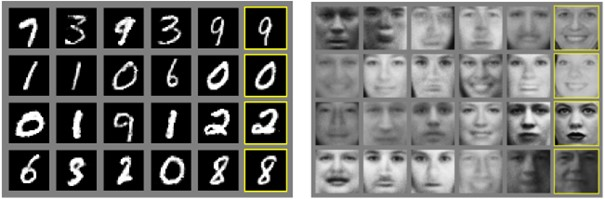
\includegraphics[width=1\textwidth]{gan_results.jpg}
    \caption[Generated numbers and faces from the work of Goodfellow et al.]{Generated results using the MINST and TFD dataset from the work of Goodfellow et al.}
    \label{fig:ganresults}
\end{figure}

\subsection{Deep Convolution Generative Adversarial Networks}
To overcome the difficulties of modifying GANs using the CNN architecture to work 
with images, DCGANs removes fully connected hidden 
layers for fractional-strided convolutions in the generator and strided convolutions 
in the discriminator \cite{AlR16}. This essentially swaps the optimization problem into learning 
an effective kernel that is able to generate the desired distribution. Spatial pooling 
functions are replaced since global average pooling increases model stability at the 
cost of convergence speed. To optimize this trade off, the convolutional features are 
directly connected to the input and output layer of both the networks. After each 
convolutional layer, Leaky Rectified Linear Unit (Leaky ReLU) activation functions are used in the 
generator and discriminator as it allows for back-propagation even for negative input 
values except for the output layer of the generator, which uses the Tanh function to 
quickly learn to saturate the color space for the training distribution completely.
\begin{figure}[H]
    \centering
    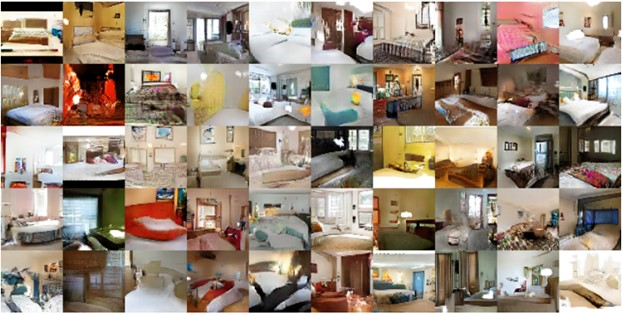
\includegraphics[width=1\textwidth]{dcgan_results.jpg}
    \caption[Generated bedrooms from the work of Radford et al.]
{Generated bedrooms using the LSUN dataset after five epochs of training from the work of Radford et al.}
    \label{fig:dcganresults}
\end{figure}
\newpage

\subsection{Wasserstien Generative Adversarial Networks with Gradient Penalty}
\label{wgan-gp}
As DCGANs use a Binary Cross Entropy Loss function instead of the KL divergence 
to minimize the Jensen Shannon divergence in GANs, they suffer from the 
generator’s tendency to converge towards a singular solution to fool the 
discriminator (mode collapse) and vanishing gradients of discriminator predictions 
when trained to optimality. This is potentially from the generator’s parameter space 
not being continuous and is addressed by using Wasserstein-1 distance to express 
the dissimilarity between two distributions. This provides the minimum cost to rearrange 
one distribution to another \cite{MaA17}. This Wasserstien GAN (WGAN) reconstructs the 
min-max game using the Kantorovich-Rubinstein duality with sample $\tilde{x}$ 
belonging to the generated distribution $\mathbb{P}_{g}$ and $x$ to the real distribution $\mathbb{P}_{r}$.
\begin{equation} \label{eq:wganopt}
\min_{G}\max_{D\in\mathcal{D}}\mathop{{}\mathbb{E}}_{x\sim\mathbb{P}_{r}}[D(x)]- \mathop{{}\mathbb{E}}_{\tilde{x}\sim\mathbb{P}_{g}}[D(\tilde{x})]
\end{equation}
Another variation added to the traditional WGAN consists of a more robust loss 
function that accounts for higher order moments of the data distribution by 
introducing a penalty on the gradient norm for random samples $\hat{x}$. Unlike 
the k-Lipshitz constraint previously implemented through weight clipping, that biases the 
critic towards simpler functions, this gradient penalty enforces a 1-Lipshitz 
constraint on the gradient norm of the critic’s output to its input \cite{IsG17}.
\begin{equation} \label{eq:wganloss}
L = \mathop{{}\mathbb{E}}_{\tilde{x}\sim\mathbb{P}_{g}}[D(\tilde{x})] - \mathop{{}\mathbb{E}}_{x\sim\mathbb{P}_{r}}[D(x)] + \lambda\mathop{{}\mathbb{E}}_{\tilde{x}\sim\mathbb{P}_{\tilde{x}}}[(\|\nabla_{\tilde{x}}D(\tilde{x})\|_{2}-1)^2]
\end{equation}
DCGANs also normalize each feature independently across the batch to 
prevent the generator from collapsing all samples to a single point before every layer 
(except the generator’s output layer and critic’s input layer as it results in sample 
oscillation and model instability) but doing this changes the problem from individual 
mapping to mapping the entire batch for the discriminator. Thus, batch 
normalization is substituted with layer normalization in the critic since it does not 
introduce correlations between examples and the penalized training objective is now 
calculated using the norm of the critic’s gradient with respect to each input 
independently. 
\newpage

\subsection{U-Net}
U-Nets are convolutional classification networks consisting of a contracting path to capture context followed 
by a symmetrically expanding path that enables localization \cite{OlR15} and concatenates the corresponding 
features from the contracting path. The network’s loss is computed with a pixel-wise softmax through the 
use of a cross entropy loss function. The activation $a_{k}$ for the set of classes $K$ at the pixel position 
$x$ is used to approximate a maximum function $p_{k}(x)$ that is meant to identify the true class for 
the image by bringing the results of the class with the maximum activation closer to 1 
while dropping the output for the remainder of the classes near to 0.
\begin{equation} \label{eq:unetact}
p_{k}(x) = exp(a_{k}(x))/(\sum_{k'=1}^K exp(a_{k'}(x)))
\end{equation}
\begin{equation} \label{eq:unetloss}
E = \sum_{x\in\omega} w(x)log(p_{\ell(x)}(x))
\end{equation}
The cross entropy then penalizes at each position the deviation of the activation $p_{\ell(x)}$ 
from the true label $\ell$ for each pixel and uses a pre-computed weight map $w$ to give more 
importance to certain pixels, compensating for the different pixel frequencies in the dataset 
while the network is training. The initial parameter weights are drawn from a Gaussian distribution 
such that features have approximately unit variance. It is optimized through minimizing the Euclidean 
distance by averaging all plausible outputs with high momentum to ensure that the current optimization 
step is more based towards previously seen training samples.

\subsection{Conditional Generative Adversarial Networks}
Unlike conventional GANs, cGANs use a U-Net based architecture as its generator to 
perform image to image translations by mapping input images $x$ towards the 
desired output images $y$ using the noise $z$. It employs an $L1$ loss that can accurately 
capture low frequency information but produces blurry results since it cannot capture its high frequency 
sharpness. Thus, a Patch classifier is also incorporated which only penalizes structure at the scale 
of image patches to model high frequency structures. 
\begin{equation} \label{eq:l1loss}
L_{L1}(G) =  \mathop{{}\mathbb{E}}_{x,y,z}[\|y-G(x,z)\|_{1}]
\end{equation}
\begin{equation} \label{eq:patchloss}
L_{cGAN}(G,D) =  \mathop{{}\mathbb{E}}_{y}[logD(x,y)] +  \mathop{{}\mathbb{E}}_{x,z}[log(1-D(x,G(x,z)))]
\end{equation}
This tackles the issues of blurriness by classifying patches of an image as real or generated and running 
the discriminator convolutionally across the image, averaging all its responses while assuming pixels 
separated by more than a set patch diameter are independent \cite{PhI17}. As such a network 
requires low-level information shared between the input and output, it uses small 
batches with high momentum while retaining batch normalization and dropout. The final objective is
realized as a min-max game similar to that of the GAN with the inclusion of conditional inputs in both of its networks 
and an additional $L1$ loss that is amplified through $\lambda$.
\begin{equation} \label{eq:cganminmax}
\min_{G}\max_{D}L_{cGAN}(G,D)+\lambda L_{L1}(G)
\end{equation}
\begin{figure}[H]
    \centering
    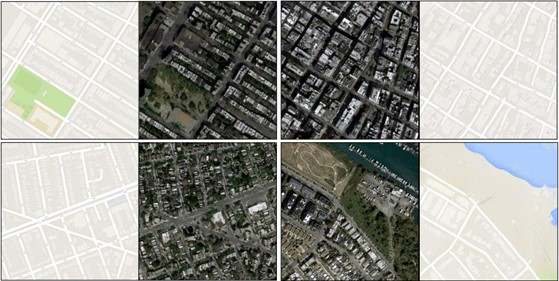
\includegraphics[width=1\textwidth]{cgan_results.jpg}
    \caption[Generated Google Maps images from the work of Isola et al.]{Generated results on Satellite and translated images from Google Maps from the work of Isola et al.}
    \label{fig:cganresults}
\end{figure}

\chapter{Representation and Prior Design}
\label{ch:representation and prior design}%

\section{DOOM}
In this thesis, the experiments are built around the game Doom \cite{IdS93} which was pivotal in 
the establishment of the FPS genre, putting forward novel techniques for 3D graphics as well as 
initiating support for custom modifications in its level format through its ports. It spawned 
dozens of copies, now called  ‘DOOM Clones’ with Figure~\ref{fig:doomclones} showing that more 
than half the code base is cloned in certain older titles \cite{YaC14}. As one of the earliest 3D games, 
DOOM is a viable subject due to its many freely accessible custom levels that has been developed by 
the community over the years which are still tracked by websites such as ‘Doomworld’. It also benefits 
from its simpler 2D representation despite its 3D player environment, drastic simplifying the structures used to model 
and subsequently reducing the computational costs with its reduced sample space. This also benefits 
from widely available and detailed documentations, enabling it to be easily parsed and reverse engineered.
\begin{figure}[H]
    \centering
    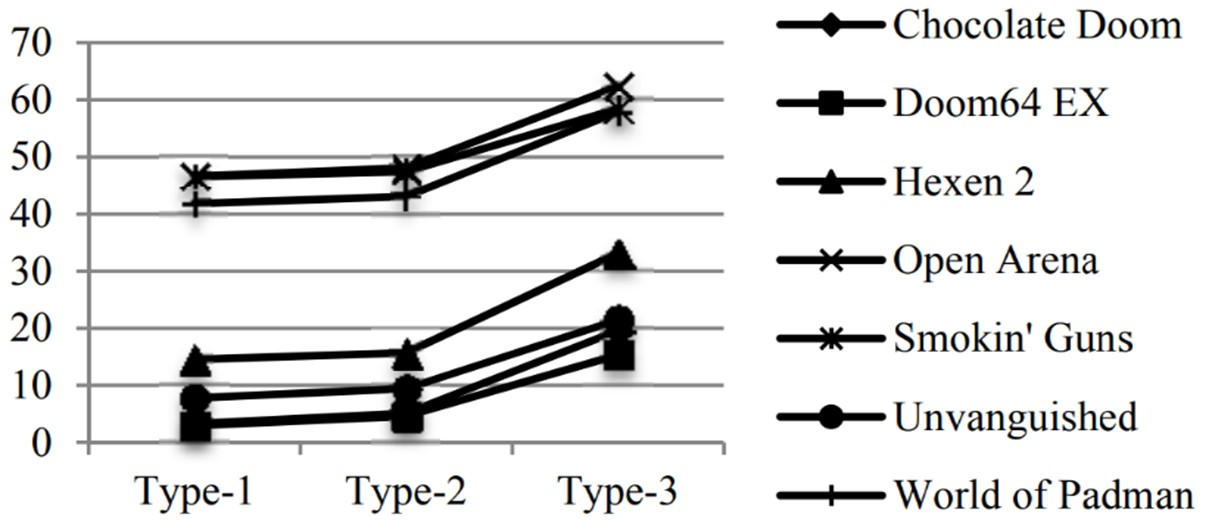
\includegraphics[width=0.7\textwidth]{doom_clones.jpg}
    \caption[Cloned lines of code for C-based from the work of Chen et al.]{Percentage of Total Cloned Lines of Code with exact code clones (Type-1), similar code fragment with only different token names (Type-2) and similar algorithms (Type-3) from the work of Chen et al.}
    \label{fig:doomclones}
\end{figure}

\section{WAD}
\subsection{Format}
Levels in DOOM are stored using the ‘.WAD’ format and contain all the necessary 
information for the DOOM engine to create the level \cite{MaF94}. The game was sold with 9 
official levels which are Internal WADs or IWADs. These explicitly define each and every  
feature such as terrain and game objects as well as any graphics and sound required 
by the level. The dataset used in this experiment are solely Patch WADs or PWADs
which are levels built by the community through map editors such as DOOM 
Builder and contain custom content or modifications that either add to or replace 
those already present in the originally referenced IWADs.

\subsection{Structure}
Each WAD is composed of byte data ordered as a sequence of lumps which is used 
to describe the feature to the DOOM Engine. It is preceded by a header that provides the 
WAD’s metadata and is succeeded by a directory containing metadata on every 
lump.

\newcolumntype{L}[1]{>{\justifying\let\newline\\\arraybackslash\hspace{3pt}}m{#1}}
\newcolumntype{C}[1]{>{\centering\let\newline\\\arraybackslash\hspace{3pt}}m{#1}}
\begin{table}[H]
\centering 
\begin{tabular}{ |C{2cm}|C{2cm}|C{1.5cm}|C{3cm}|L{5cm}| }
\hline
\textbf{Section Length (bytes)} & \textbf{Section Name} & \textbf{Field Size (bytes)} & \textbf{Field Name} & \multicolumn{1}{c|}{\textbf{Description}} \\
\hline
\multirow{3}{*}{12} & \multirow{3}{*}{Header}& 4 & Identification & ‘PWAD’ or ‘IWAD’ in ASCII\\ \cline{3-5}
 & & 4 & Number of Lumps & Integer value of lumps included in WAD\\ \cline{3-5}
 & & 4 & Table Offset & Integer pointer to resource dictionary\\ 
\hline
Variable & Lumps & - & Lump Data & Lumps stored as a byte stream\\
\hline
\multirow{3}{4em}{\centering16 * Number of Lumps} & \multirow{3}{*}{Directory}& 4 & Lump Position & Pointer to respective lump data\\ \cline{3-5} 
 & & 4 & Lump Size & Size of respective lump in bytes\\ \cline{3-5}
 & &  8 & Lump Name & Lump Name in ASCII\\ 
\hline
\end{tabular}
\\[10pt]
\caption{Sections of a WAD as seen in the work of Giacomello et al.}
\label{table:wadsections}
\end{table}


\subsection{Contents}
All the information that is used to define a level can be found within their respective
 lumps with each designated to a specific component of the level structure. The lumps 
defined in the Table~\ref{table:uniquelumps} and Table~\ref{table:derivablelumps} represent 
all of the mandatory lumps that should be present in every WAD to be deemed acceptable by the 
DOOM engine. Most lumps partition its entries into a set of fields with multiple entries in different lumps 
sometimes used to define a single entity. It also provides the necessary metadata that is used to 
signify special effects through fields allotted for flags that are present in all the unique 
lumps mentioned except for name and vertexes.

\begin{table}[H]
\centering 
\begin{tabular}{ |C{2.5cm}|L{8cm}|C{1.5cm}|C{1.5cm}|}
\hline
\textbf{Lump Name} &\multicolumn{1}{c|}{\textbf{Description}} & \textbf{Entry Size (bytes)} & \textbf{No. of Fields} \\
\hline
NAME & The IWAD level name as an ‘ExMy’ label where ‘x’ is the episode number and ‘y’is the mission 
number & 2 & 1 \\
\hline
THINGS & A list of every game object present that is not a wall, pavement or door, identified using 
an index with its position and orientation & 10 & 5 \\
\hline
LINEDEFS & A list of every line needed to signify all the walls, steps, and invisible boundaries such as 
event triggers that shape the level & 14 & 7 \\
\hline
SIDEDEFS & A list of referenced wall textures, specifying the sector that it faces and implicitly 
defining the sector's boundaries & 30 & 6 \\
\hline
VERTEXES & A list of x and y map coordinates that are referenced by linedef entries to create shapes on 
the map & 4 & 2 \\
\hline
SECTORS & A list of closed areas with the same floor and ceiling textures as well as height. Additional 
fields describe its lighting and the floor’s special effects that usually damage the player & 26 & 7 \\
\hline
\end{tabular}
\\[10pt]
\caption{Unique mandatory lumps in a WAD}
\label{table:uniquelumps}
\end{table}
\newpage

The level building process begins through the designation of an individual sector 
and iteratively laying out its components until all the sectors are rendered. Sectors are 
constructed using the relevant linedefs which are obtained through associated sidedef entries that 
reference the respective sector. Linedefs are defined using two entries from the 
vertex lump and can either mention only a right sidedef for boundary walls or also a left sidedefs when 
connecting two sector which can both be transparent to act as triggers using the corresponding flag . 

There are certain constraints to the formation of lumps such 
as the presence of exactly one name lump in every WAD and the inability to render 
sectors above or below another since it uses a 2D map. Other functional lumps can be
derived from the former using 3rd party software and serve to speed up the rendering 
process by avoiding runtime computation. All the lumps mentioned here except reject 
are mandatory for the engine to be able to build the level. These lumps include:

\begin{table}[H]
\centering 
\begin{tabular}{ |C{2.5cm}|L{8cm}|C{2cm}|C{1.5cm}|}
\hline
\textbf{Lump Name} &\multicolumn{1}{c|}{\textbf{Description}} & \textbf{Entry Size (bytes)} & \textbf{No. of Fields} \\
\hline
SEGS & A list of wall segments comprising either a part or all of a linedef entry which are combined 
to form the various sub-sectors & 12 & 6 \\
\hline
SSECTORS & A list of sub-sectors which are the smallest undivided spaces incapable of obstructing 
the visibility of other walls within it & 4 & 2 \\
\hline
NODES & Branches in a 2D binary space partition tree sorting the view order of each sub-sector 
which speeds up the rendering process & 28 & 8 \\
\hline
BLOCKMAP & Pre-computed collision detection map without which objects and walls within the 
level cannot interact with any another & - & - \\
\hline
REJECT & Table to determining if an agent can ascertain the players location for visibility calculations  
used to optimize AI routines & 1 & 8 \\
\hline
\end{tabular}
\\[10pt]
\caption{Derivable mandatory lumps in a WAD}
\label{table:derivablelumps}
\end{table}
\newpage

These lumps speed up the rendering process by using a graph to represent the 
overall structure of the level and decide what needs to be shown by taking into 
account the player position and sorting the sub-sectors that are supposed to be 
visible to user. This is achieved by using the sub-sectors composed of segments as 
nodes in the graph that are rearranged every time the player moves through 
partition lines that divide the map and get iteratively smaller for each child until 
all sub-sectors have been encompassed.

Some of the derivable lumps have more unique structures such as the reject which 
expects byte sized entries with each bit representing visibility from a sector and the 
final byte padded to meet the size requirement. The blockmap on the other hand is 
preceded by a header of 8 bytes which indicates the coordinates of the origin and the 
number of blocks within the grid. This is followed by the offset of each linedef entry 
and the corresponding line segments.
\begin{figure}[H]
    \centering
    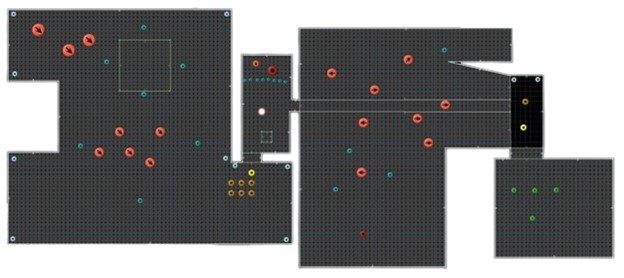
\includegraphics[width=1\textwidth]{sample_doom_builder.jpg}
    \caption[Sample DOOM PWAD visualized using DOOM Builder]{Sample DOOM PWAD visualized using DOOM Builder where orange 
indicates enemy positions, yellow represents pick-ups such as power-ups/ammunition and green is the starting position of the players}
    \label{fig:doombuilder}
\end{figure}
\newpage

\section{Giacomello’s DOOM Level Generator}
\subsection{Dataset Organization and Presentation}
WADs are converted into feature maps which function as the training data for the 
neural network. This is done by translating extracted byte data by means of a custom 
parser and composing them into local data structures for the aforementioned lumps. 
By focusing on the minimum requirements necessary for creating a DOOM level, the 
parsed dataset is limited to 4 feature maps which represent the level topology as well 
as its functional components. To this end, the wall, floor, and its height proved
capable of accurately representing the level layout while the things map handles the 
presence of gameplay elements. After parsing the WAD, relevant coordinates
for each map are marked on separate matrices. The dimensions of this matrix are 
allocated based on the length and width of the given map, scaled down from its 
original size by the radius of the smallest function object, in this case by 32 times. 

The level shape is sketched out via sectors through finding all sidedefs with the same
number in the sector field and obtaining all the linedefs that reference those sidedefs. 
The retrieved list of linedefs is used to identify the pertinent vertices which are then 
adjusted for the new scale of the map. The wall map is outlined by drawing lines 
between the referred vertices for each linedef only if it contains at least one sidedef 
that is not transparent. The height map is computed sector wise by extrapolating the 
perimeter given by these lines and iteratively traces out the respective polygons that 
envelope the area containing that sector. The floor map is obtained by creating a 
mask of the positive value in the height map while the things map uses the scaled 
coordinates to encode pixels with values from the things type dictionary. 

A further set of scalar features such as the ratio between the level area and its convex 
hull, mean room size, largest room size, room count, diameter of circle with the same 
level area, length of the longest and shortest axis of the level as well as the skewness 
and peak sharpness in the pixel distance distribution from its closest wall are also 
computed and appended to the maps as part of the dataset. This is done in order to 
provide some degree of control over the generation process as they are easily 
extracted and impervious to noise. The dataset is then stored as Tensorflow records 
to avoid recalculation.
\begin{figure}[H]
    \centering
    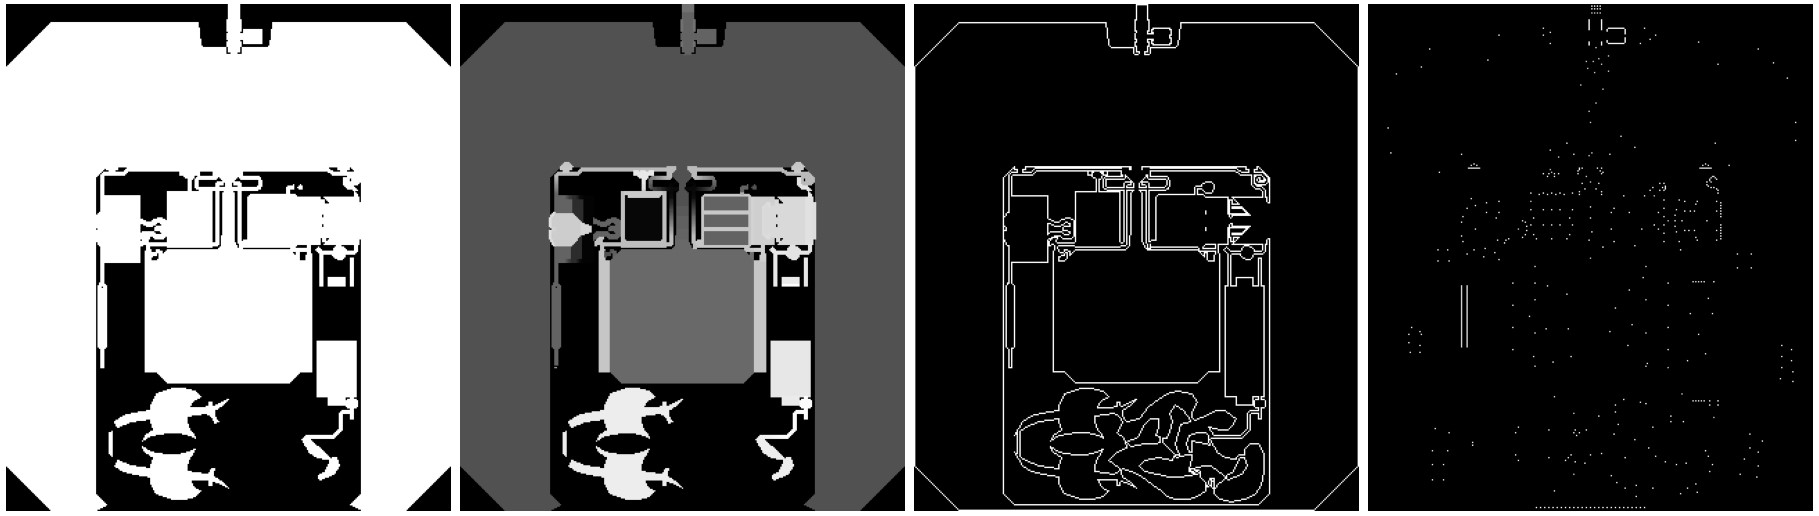
\includegraphics[width=1\textwidth]{old_feature_maps.jpg}
    \caption[Feature maps of a sample level]{Floor map, Height map, Wall map, and Things map (from left to right) of a 
sample level}
    \label{fig:oldfeaturemaps}
\end{figure}
The feature maps shown in Figure 3.3 represent the level in its bare minimum and 
are used to derive all the mandatory lumps required to furnish a level while 
delivering the gameplay envisaged by the genre. The features maps are engineered
as such:
\begin{itemize}
\item FLOOR MAP: Depicts the floor layout of the level by segregating the 
available space into the portion that lies within bounds of the level using pixel 
values of 255 to denote them and leaves that which remain with a pixel value 
of 0.
\item HEIGHT MAP: Marks the height of various sections of the map by encoding 
pixel values in gradients for segregating each sector with a maximum value of 
255 and those outside the bounds of the floor map as 0.
\item WALL MAP: Compartmentalizes the level into separate rooms and visualizes 
the points of access for each of the rooms by tracing the positions of the walls 
used to partition it. Walls are marked with a pixel value of 255 while the rest 
are left with a pixel value of 0.
\item THINGS MAP: Indicates the position of the game objects on the map by 
identifying the type of object through pixel values assigned using the id 
allotted to it in the things type dictionary while the absence of objects is 
represented as 0.
\end{itemize}
\newpage

\subsection{System Architecture}

\begin{wrapfigure}{l}{0.6\textwidth}
    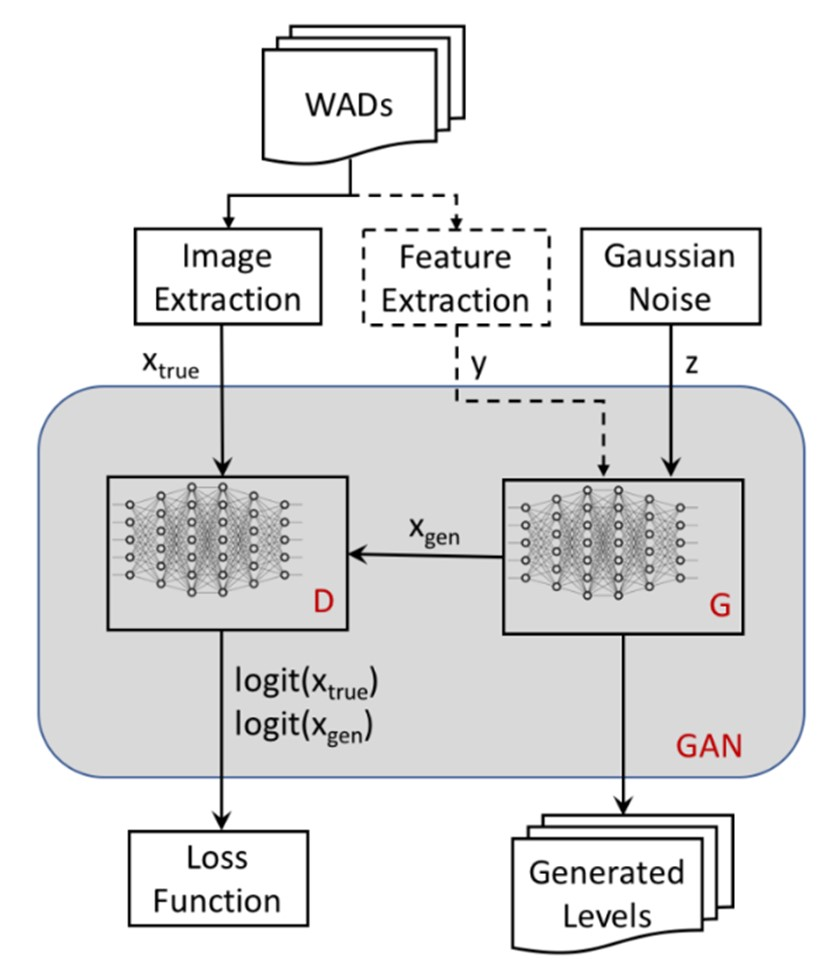
\includegraphics[width=0.6\textwidth]{cWGAN.jpg}
    \caption[Conditional WGAN-GP architecture from the work of Giacomello et al.]{Conditional WGAN-GP architecture used for the generation DOOM levels from the work of Giacomello et al.}
    \label{fig:cwgan}
\end{wrapfigure}

Giacomello approaches the problem of procedurally generating DOOM levels by means of a Conditional 
Wassertien GAN with a Gradient Penalty \cite{EdG18}. By rescaling the feature maps extracted from the 
TFrecords into the same shape of 128 by 128 pixels, the generator is trained on a normalized version of 
the dataset which is further enlarged by including three more orientations by rotating the maps 
in multiples of 90-degree. The extracted input scalars called ‘Feature Vectors’ are also 
appended to the feature maps to correlate the parameter to their respective level. 

The generative network has five hidden layers which comprise of one linear layer followed by 
convolutional layers with a final convolutional output layer applying a sigmoid activation 
function as it better coincides with the target format. It uses the feature vectors 
accompanied by a gaussian noise vector as input and learns its distribution while the 
critic uses the real feature maps and the generated ones to grasp the differences
between them given those feature vectors. The model’s predictions are then 
evaluated based on the Wasserstien distance from its expected value. The parameters 
are then adjusted using an Adam Optimizer with the generated levels compared 
using metrics such as corner count, structural similarity index and encoding error to 
assess the quality of the developed architecture.

\subsection{WAD Generation}
Once the network is capable of generating maps recognizable as DOOM levels, a 
custom WAD writer is used to reverse engineer the matrices into lumps of byte data 
representing the mandatory components of a PWAD. By using the floor, wall, height, 
and things feature maps, it prepares the level layout by reconstructing the 
information into an undirected weighted graph. This is done through computing the 
respective room maps by means of a segmentation algorithm to compartmentalize 
sections of the walkable area of the level. The graph is then constructed outwards 
from the center and is decorated with various features while keeping the textures 
constant. 

Level paths that can be traversed are collected using a minimum spanning trees 
algorithm on the graph from the section of the level with the least entrances which is 
used as the starting position of the level. Based on the computed solutions, an exit 
trigger is generated at the end of the longest floor path. Once the graph is complete, 
its nodes are translated into their respective lumps by scaling up each of the 
coordinates by 64 before it is finally committed with a level name and generated as a 
WAD. Four texture entries are required in all such PWADs for DOOM to run 
properly which are $‘FLOOR4\char`_8$’, ‘$SFLR6\char`_1$’, ‘$MFLR8\char`_4$’, and ‘$FLOOR7\char`_2$’. The first 
three are needed as backgrounds for the episode end texts. The last is what is shown 
outside the border of the display window when not being run in full screen.

\subsection{Drawbacks}
Due to the use of interpolation techniques to resize the image into identical sizes, 
the information within the images is not exactly translated when performing such 
transformations. Effects of distortion and blurring can be addressed or ignored 
during the dataset preparation for the topological maps as the variation is consistent 
in the height map while the floor and wall maps are indifferent to exact pixel values. 
Sparse images such as the things map that depend on the pixel encoded values on the other hand are 
contorted beyond permissible levels of tolerance, making it to be difficult to 
maintain its integrity. In the case of the things map, this has the effect of pixels taking 
on the value of other objects, coercing them towards objects with lower assigned ids. 
Multiple objects close together also get overlooked when larger maps are scaled 
down from their original size based on the order the object is presented with the 
WAD. This is due to compacting the level space which results in large units of area 
converging into a single pixel and the indiscriminate superseding by the last object in 
the list regardless of category, further dissociating the relations between object types.
\begin{figure}[H]
    \centering
    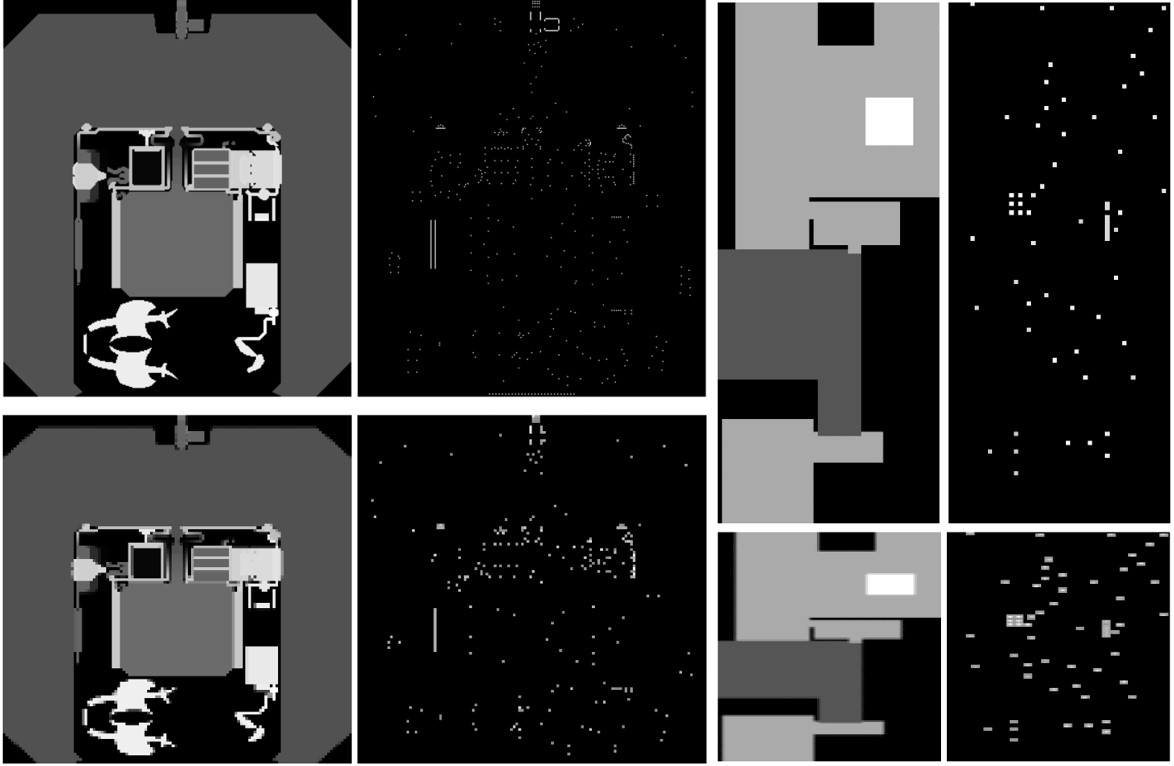
\includegraphics[width=1\textwidth]{feature_map_mistakes.jpg}
    \caption[Resized feature maps comparison]{Height and Things maps (From left to right) of the sample levels (above) 
compared to its resized counterpart (below)}
    \label{fig:featuremapistakes}
\end{figure}
Maps smaller than the target size of 128 by 128 pixels meanwhile must be 
enlarged to compensate for the lack of area which leads to objects being represented 
through the multiple surrounding pixels, further deteriorating the quality of the 
map. It also leads to large empty spaces throughout the level which can throw of the 
networks ability to learn and populate the level space completely.

There are bugs encountered in the generation process as disconnected sections of the 
level are inaccessible and the objects present within these portions of the level do not 
meaningfully contribute in any way to the actual proportions of the category types. If 
the player spawns in a section that has a greater population of monsters while 
another detached section has more ammunition, it presents the player with little to 
no opportunity to exploit the totality of resources available. Attached segments can 
also be inaccessible when the connecting corridors are too small to traverse, only 
allowing the player to peek through which is detrimental to gameplay.

\section{Improved Feature Map Extraction}
To alleviate some of the problems encountered, modifications have been made to
Giacomello’s WAD Editor to parse the WADs for a better representation of the
sufficient subset of unique feature used to design a level. From  Figure~\ref{fig:areadist}, it can be 
noted that most maps lie below 15000 units in both dimensions from the figure. The 
parsed maps are now scaled down to 256 by 256 pixels with levels below 15000 units 
being relatively padded by two row or columns for every 300 units smaller than the 
mentioned limit in its respective dimension to preserve objects density. Although 
there is still some overlap among game objects, integrity of pixel values is ensured by 
using only coordinate rescaling instead of resizing throughout the entire process.
\begin{figure}[H]
    \centering
    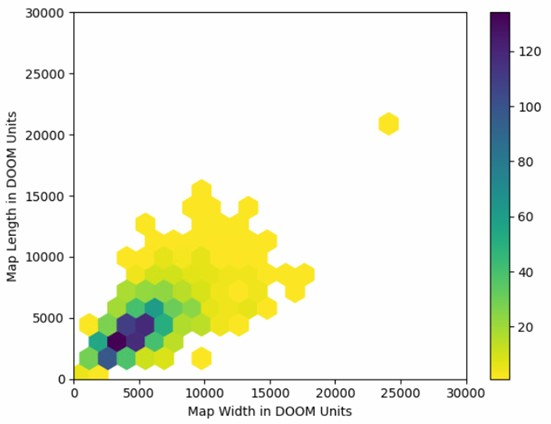
\includegraphics[width=1\textwidth]{area_distribution.jpg}
    \caption[Area distribution of the filtered dataset]{Area distribution of the filtered dataset}
    \label{fig:areadist}
\end{figure}
While retaining the topological maps, the things map has been further divided into 
their individual category maps to provide a more coherent context for the system to 
process. Objects of the respective category are designated an id, acquired by 
arranging them in the order of significance of the effect it has on gameplay. Only 
functional elements that are required to fully experience the game have been factored 
in and can be recombined to recreate the thingsmap. The categories included are
monsters, ammunition, power-ups, artifacts, and weapons.
\begin{figure}[H]
    \centering
    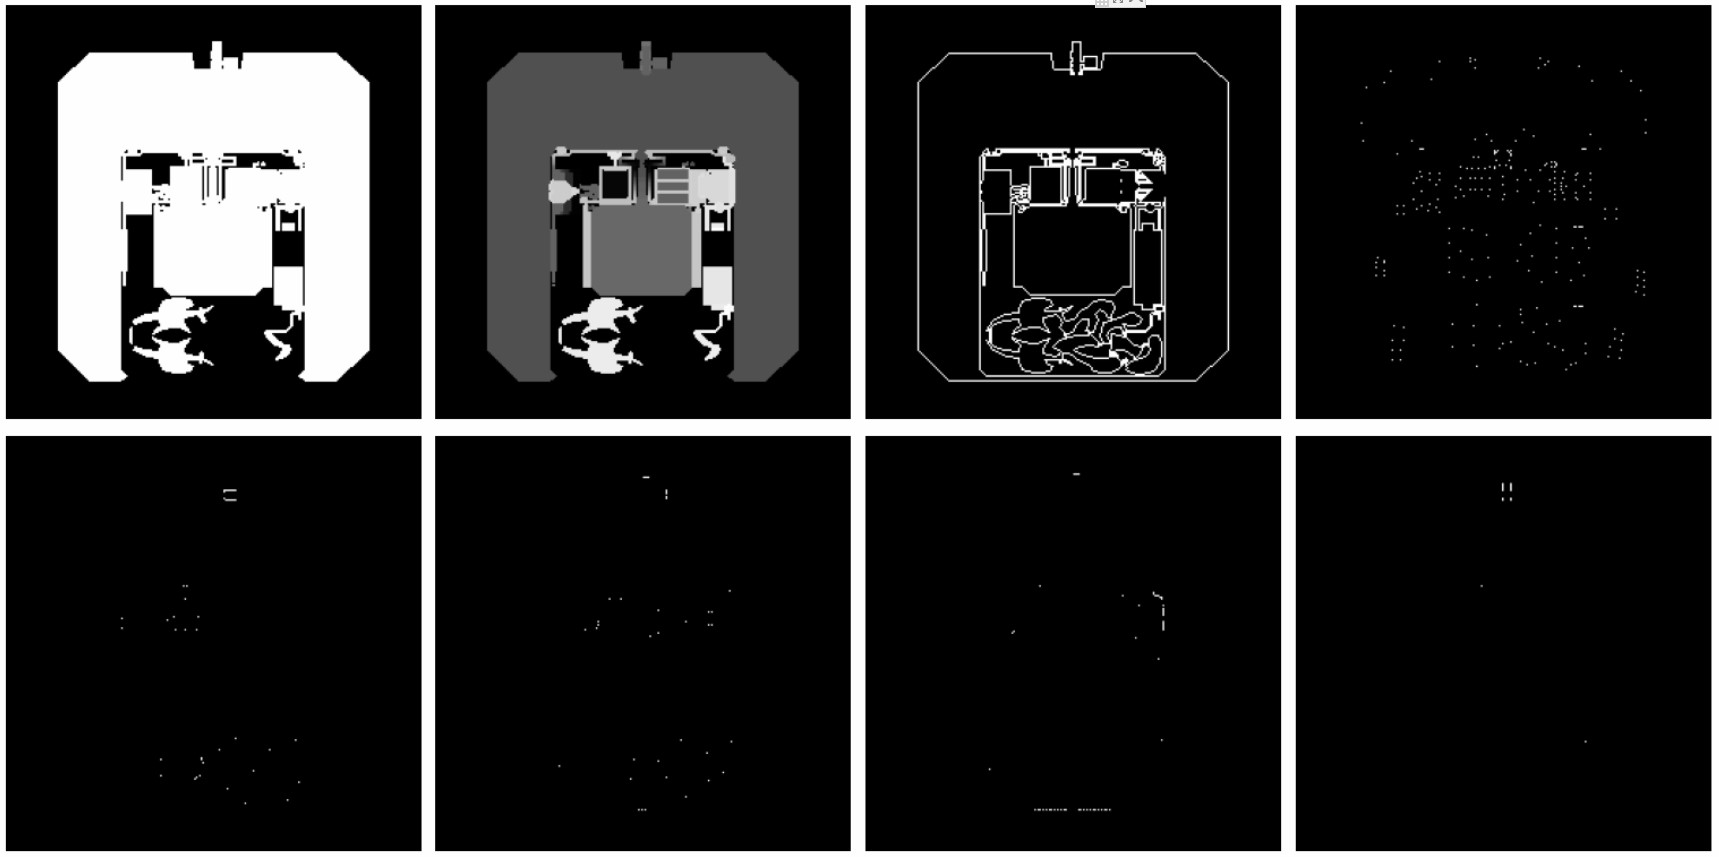
\includegraphics[width=1\textwidth]{new_feature_maps.jpg}
    \caption[Updated feature maps of a sample level]{Floor, Height, Wall, Monsters, Ammunition, Powerups, Artifacts and 
Weapons map (From left to right, top to bottom) of the sample level using coordinate rescaling}
    \label{fig:newfeaturemaps}
\end{figure}
The newly added set of feature maps apart from the included floor, height and wall 
maps from the previous design are:
\begin{itemize}
\item MONSTERS MAP: Assigns the respective positions of enemies with the pixel 
value corresponding to its monster id and 0 representing its absence.
\item AMMUNITIONS MAP: Assigns the respective positions of ammunition used by 
the various weapons with the pixel value corresponding to its ammunition id 
and 0 representing its absence.
\item POWERUPS MAP: Assigns the respective positions of armor and first aid with 
the pixel value corresponding to its powerup id and 0 representing its 
absence.
\item ARTIFACTS MAP: Assigns the respective positions of specialized abilities 
with the pixel value corresponding to its artifact id and 0 representing its 
absence.
\item WEAPONS MAP: Assigns the respective positions of the various weapons 
with the pixel value corresponding to its weapon id and 0 representing its 
absence.
\end{itemize}

Mentioned in Table~\ref{table:gameobjs1} and Table~\ref{table:gameobjs2} are the list of game objects that have been taken into 
consideration as they provide a functional value to the setting of the game. Apart 
from the start position of the player, the remainder of the objects are generated using 
the implemented model.

\begin{table}[H]
\centering 
\begin{tabular}{ |C{1cm}|C{2cm}|C{5.5cm}|C{2.5cm}|C{2cm}|}
\hline
\textbf{Id} & \textbf{Things Type Id} & \textbf{Description} & \textbf{Category} & \textbf{Category Id} \\
\hline
1 & 0 & Empty & - & 0\\
2 & 3 & Player 1 Start & other & 1\\
3 & 75 & Arachnotron & monster & 11\\
4 & 76 & Arch-Vile & monster & 14\\
5 & 77 & Baron of Hell & monster & 16\\
6 & 78 & Cacodemon & monster & 9\\
7 & 79 & Chaingunner & monster & 7\\
8 & 81 & Cyberdemon & monster & 17\\
9 & 82 & Demon & monster & 4\\
10 & 83 & Former Human Trooper & monster & 3\\
11 & 84 & Former Human Sergeant & monster & 5\\
12 & 85 & Hell Knight & monster & 15\\
13 & 86 & Imp & monster & 1\\
14 & 87 & Lost Soul & monster & 8\\
15 & 88 & Mancubus & monster & 13\\
16 & 89 & Pain Elemental & monster & 10\\
17 & 90 & Revenant & monster & 12\\
18 & 91 & Spectre & monster & 6\\
19 & 92 & Spider Mastermind & monster & 18\\
20 & 93 & Wolfenstein SS & monster & 2\\
21 & 94 & Ammo Clip & ammunitions & 2\\
22 & 95 & Box of ammo & ammunitions & 6\\
23 & 96 & Box of rockets & ammunitions & 7\\
24 & 97 & Box of shells & ammunitions & 5\\
25 & 98 & Cell charge & ammunitions & 4\\
\hline
\end{tabular}
\\[10pt]
\caption{List of relevant game objects with category ids (1 of 2)}
\label{table:gameobjs1}
\end{table}

\begin{table}[H]
\centering 
\begin{tabular}{ |C{1cm}|C{2cm}|C{5.5cm}|C{2.5cm}|C{2cm}|}
\hline
\textbf{Id} & \textbf{Things Type Id} & \textbf{Description} & \textbf{Category} & \textbf{Category Id} \\
\hline
25 & 98 & Cell charge & ammunitions & 4\\
26 & 99 & Cell charge pack & ammunitions & 8\\
27 & 100 & Rocket & ammunitions & 3\\
28 & 101 & Shotgun shells & ammunitions & 1\\
29 & 102 & BFG9000 & weapons & 7\\
30 & 103 & Chaingun & weapons & 3\\
31 & 104 & Chainsaw & weapons & 1\\
32 & 105 & Plasma Rifle & weapons & 6\\
33 & 106 & Rocket Launcher & weapons & 5\\
34 & 107 & Shotgun & weapons & 2\\
35 & 108 & Super shotgun & weapons & 4\\
36 & 109 & Backpack & powerups & 3\\
37 & 110 & Blue armor & powerups & 5\\
38 & 111 & Green armor & powerups & 2\\
39 & 112 & Medikit & powerups & 4\\
40 & 113 & Radiation suit & powerups & 6\\
41 & 114 & Stimpack & powerups & 1\\
42 & 115 & Berserk & artifacts & 3\\
43 & 116 & Computer map & artifacts & 5\\
44 & 117 & Health potion & artifacts & 1\\
45 & 118 & Invisibility & artifacts & 8\\
46 & 119 & Invulnerability & artifacts & 9\\
47 & 120 & Light amplification visor & artifacts & 7\\
48 & 121 & Megasphere & artifacts & 6\\
49 & 122 & Soul sphere & artifacts & 4\\
50 & 123 & Spiritual armor & artifacts & 2\\
\hline
\end{tabular}
\\[10pt]
\caption{List of relevant game objects with category ids (2 of 2)}
\label{table:gameobjs2}
\end{table}

\chapter{Implementation}
\label{ch:implementation}%

\section{Dataset Procurement}
The data used to train and validate the models is obtained by scraping custom made 
doom levels from 'doomworld.com', a source mirror of Idgames Archive. A scraper 
is made to access the domain and iterate over the web pages of the available levels 
within each subcategory present excluding ‘Deathmatch’, ‘Megawads’ and ‘Ports’.
This choice has been made to avoid mixing different types of levels as player vs 
player environments are structurally different from player vs enemy environments. 
Ports has been ignored because it requires modifying the game engine to run the 
level which is complicated to characterize in a format decipherable by the model and 
stably implement into PWADs. The web scraper then downloads WADs and stores 
relevant information in a JSON file which doubles as a register to catalog the 
collection at hand. 

Among the custom levels present in Doomworld’s repository, 1969 of the available 
levels do not fall within the excluded categories mentioned above. In an effort to 
reduce the complexity of the problem, WADs containing only a single level have 
been included to ease the requirements of the system with a simpler manner of 
representation. Similarly, constraints have been placed on the levels to ensure its 
faithfulness to the genre is respected such as accepting only those that contain at least 
one monster and weapon to improve the overall consistency within the dataset. 
Finally, to forgo the intricacies that arises with teleporters, levels that have large, 
detached segments have not been included, leaving only the remaining 1279 levels
which are taken into consideration and included in the finalized dataset. The WADs 
that have been determined to meet the desired criteria are then parsed and have its 
feature maps extracted to serve as the training data for the models.
\newpage

\section{System Architecture}

\begin{wrapfigure}{l}{0.55\textwidth}
    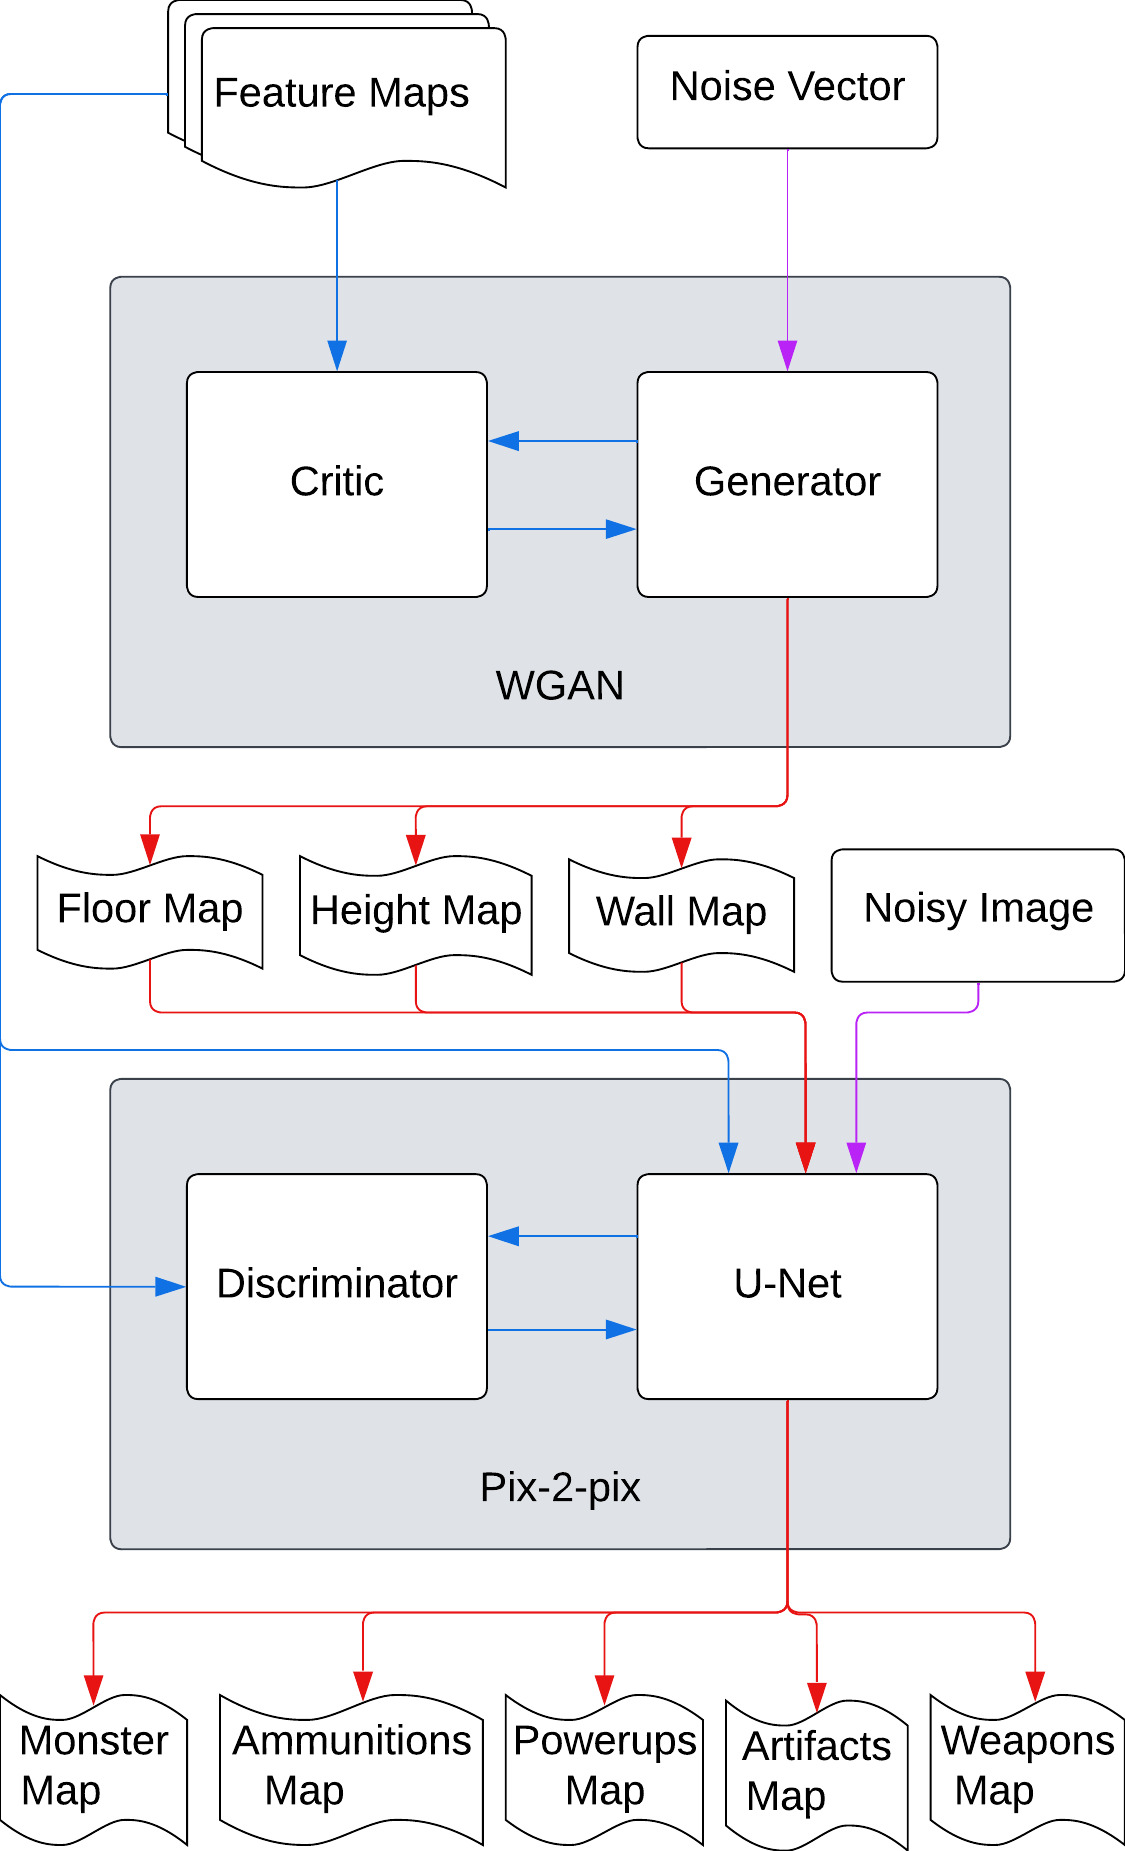
\includegraphics[width=0.55\textwidth]{hybrid_architecture.jpeg}
    \caption[Hybrid GAN architecture]{The hybrid GAN architecture where blue 
lines represent the training process, red line are used in the generation process and the purple lines are for both}
    \label{fig:hybridarch}
\end{wrapfigure}
The proposed system is a hybrid architecture consisting of a WGAN-GP and a cGAN model that are 
trained on specific feature maps to grasp particular aspects of level design. The 
WGAN-GP is provided with those pertaining to the level's topology to learn to draft coherent level 
layouts while the cGAN is taught the functional aspects of the level and uses it to spawn game 
objects in a manner that positively influences the game dynamics within the generated level. 
These networks are built using the Keras Sequential API from the Tensorflow libraries in Python 3.9.

The models are split into individual networks and are trained separately due to the size restriction on 
the memory of the GPU. During the generation process, the networks are run consecutively 
with the WGAN-GP executed first so that its results can be fed into the cGAN after certain 
post processing. The results obtained from both the networks are then concatenated together 
to attain a complete set of feature maps which are then used to manufacture the mandatory 
lumps and assembled into a WAD. The remaining lumps are procured using a 3rd party software 
and this process is explained in greater detail in the following sections.

\section{Network Components}
\subsection{Topological Generator}
The subsystem is designed using Radford and Metz’s Deep Convolutional 
Generative Adversarial Network architecture with Wasserstien distance used to 
calculate the loss as undertaken by Arjovsky et al. The generator is trained alongside 
a critic implementing alterations by Gulrajani et al. which incorporates a gradient 
penalty to its loss estimation and has the inclusion of additional training steps 
compared to that of the generator. The aim is to teach this module the topological 
structure of levels which is defined by its floor space, the enclosing wall layout, and 
the respective height of each section.

The data handled involves a random gaussian noise vector $Z$, the topological feature 
maps $X$ and the critic’s classification of the allocated map $Y$. The topological 
feature maps consist of the floormap, wallmap and heightmap images and those obtained from 
the scraped dataset represents the real distribution $X_{True}$ that the generator is to learn. 
These are used in combination with images from the generated distribution to help the critic 
determines which features needs to be extracted to correctly classify a provided image. 
The sampled feature maps $X_{Gen}$ from the generated distribution is 
procured using the generator $G$ through manipulation of the noise vector i.e.,
\begin{equation} \label{eq:wgen}
X_{Gen} = G(Z)
\end{equation}
\begin{figure}[H]
    \centering
    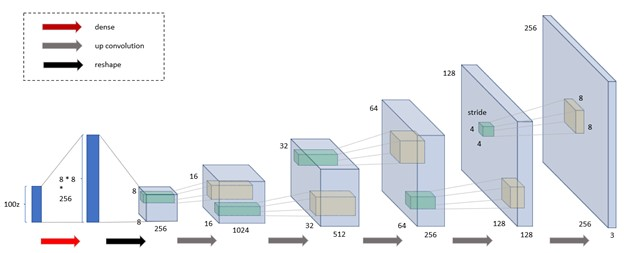
\includegraphics[width=1\textwidth]{wgan.jpg}
    \caption{Topological generator of the hybrid architecture}
    \label{fig:wgan}
\end{figure}
\newpage

The critic $C$ uses an identical architecture in the same manner with the only difference 
being that it operates on three feature maps. It processes the maps with its hidden 
layers progressively through repetitive steps of down convolution followed by layer 
normalization and Leaky ReLU activation until it is finally condensed into a single 
output assigning the map belonging either to the real distribution $Y_{True}$ and the generated 
distribution $Y_{Gen}$ to a value between 0 and 1. It is equivalent to the logits functions 
where it optimizes the critic’s prediction as follows:
\begin{itemize}
\item $Y_{Gen} = C(X_{Gen}) = Logits(X_{Gen})$ are brought closer to 0 as it indicates that the
sample is generated.
\item $Y_{True} = C(X_{True}) = Logits(X_{True})$ are brought closer to 1 which symbolizes that the 
sample is real. 
\end{itemize}

Similarly the generator is implemented without the scalar features, taking in a 100-element noise 
vector as input and manipulating the tensor length through a dense hidden 
layer to project the noise into a larger tensor. The tensor is then reshaped into a set of 
8 by 8 images which are then expanded through a series of up convolutions until the 
final output layer produces a floor, wall, and height maps for the generated level of 
pixel size 256 by 256. A sigmoid activation function is used in the output layer instead of 
the orthodox tanh function as it is more appropriate since the constraints the feature 
maps lie between have been normalized. 

\subsection{Functional Generator}
The module is based on Isola et al.’s Conditional Adversarial Network with 
modifications made to its loss function to help better extract the target distribution in 
the given circumstance. The generator’s architecture uses the three 256 by 256 pixel 
topological maps $X_{I}$ with an image of gaussian noise $Z$ of the same size and 
progressively transforms the tensors into the category maps $X_{T}$ consisting of the 
monsters, ammunition, powerups, artifacts and weapons maps. The network is 
initially trained to generate category maps $X_{T\char`_Gen}$ using the sample input $X_{I\char`_True}$ 
from the real distribution. It is then compared with the original object map $X_{T\char`_True}$ by 
the discriminator. During the generation phase, the network uses the maps $X_{I\char`_Gen}$ 
produced by the topological generator to obtain the newly generated category maps 
$X_{T\char`_GGen}$.
\begin{equation} \label{eq:ctgen}
X_{T\char`_Gen} = G(Z|X_{I\char`_True}) 
\end{equation}
\begin{equation} \label{eq:cggen}
X_{T\char`_GGen} = G(Z|X_{I\char`_Gen})
\end{equation}
The generator is trained in a method which requires it to retain its batch 
normalization even after the training process. Instead of using a tanh activation 
function for the generator output layer, a ReLU activation function 
has been used as it has proved to provide better image translation. The generator loss 
function has also been modified to account for the problem's parameters and as such 
it contains the adversarial loss i.e binary cross entropy but has the $L1$ loss substituted 
with the and mask loss which is explained in greater detail in the next section.

The discriminator classifies the target maps with its input map samples from both the
 real and generated sample distributions much like that of the WGAN-GP with the only 
differences being that it is provided with all mentioned feature maps and that is uses a 
Binary Cross Entropy loss function. Both the generator and discriminator use modules of the 
form of a convolution, followed by batch normalization and a RelU activation when upscaling 
or a Leaky ReLU while downscaling. The predictions are composed as patches which are 
calculated similar to logits and are optimized as 
\begin{itemize}
\item $Y_{Gen} = D(X_{I\char`_True}+X_{T\char`_Gen}) = Logits(X_{I\char`_True}+X_{T\char`_Gen})$ are brought closer to 0 as it indicates that the
sample is generated.
\item $Y_{True} = D(X_{I\char`_True}+X_{T\char`_True}) = Logits(X_{I\char`_True}+X_{T\char`_True})$ are brought closer to 1 which symbolizes that the sample is real. 
\end{itemize}
\begin{figure}[H]
    \centering
    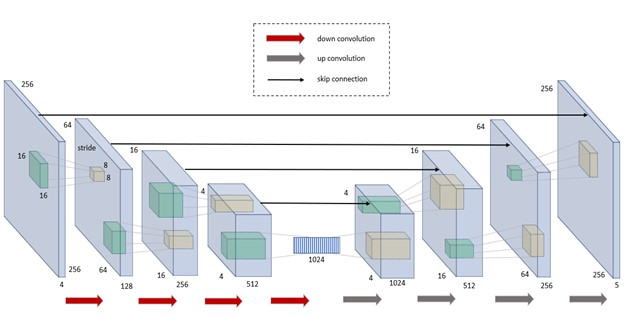
\includegraphics[width=1\textwidth]{unet.jpg}
    \caption{Functional generator of the hybrid architecture}
    \label{fig:unet}
\end{figure}

\subsection{Data Flow}
\begin{figure}[H]
    \centering
    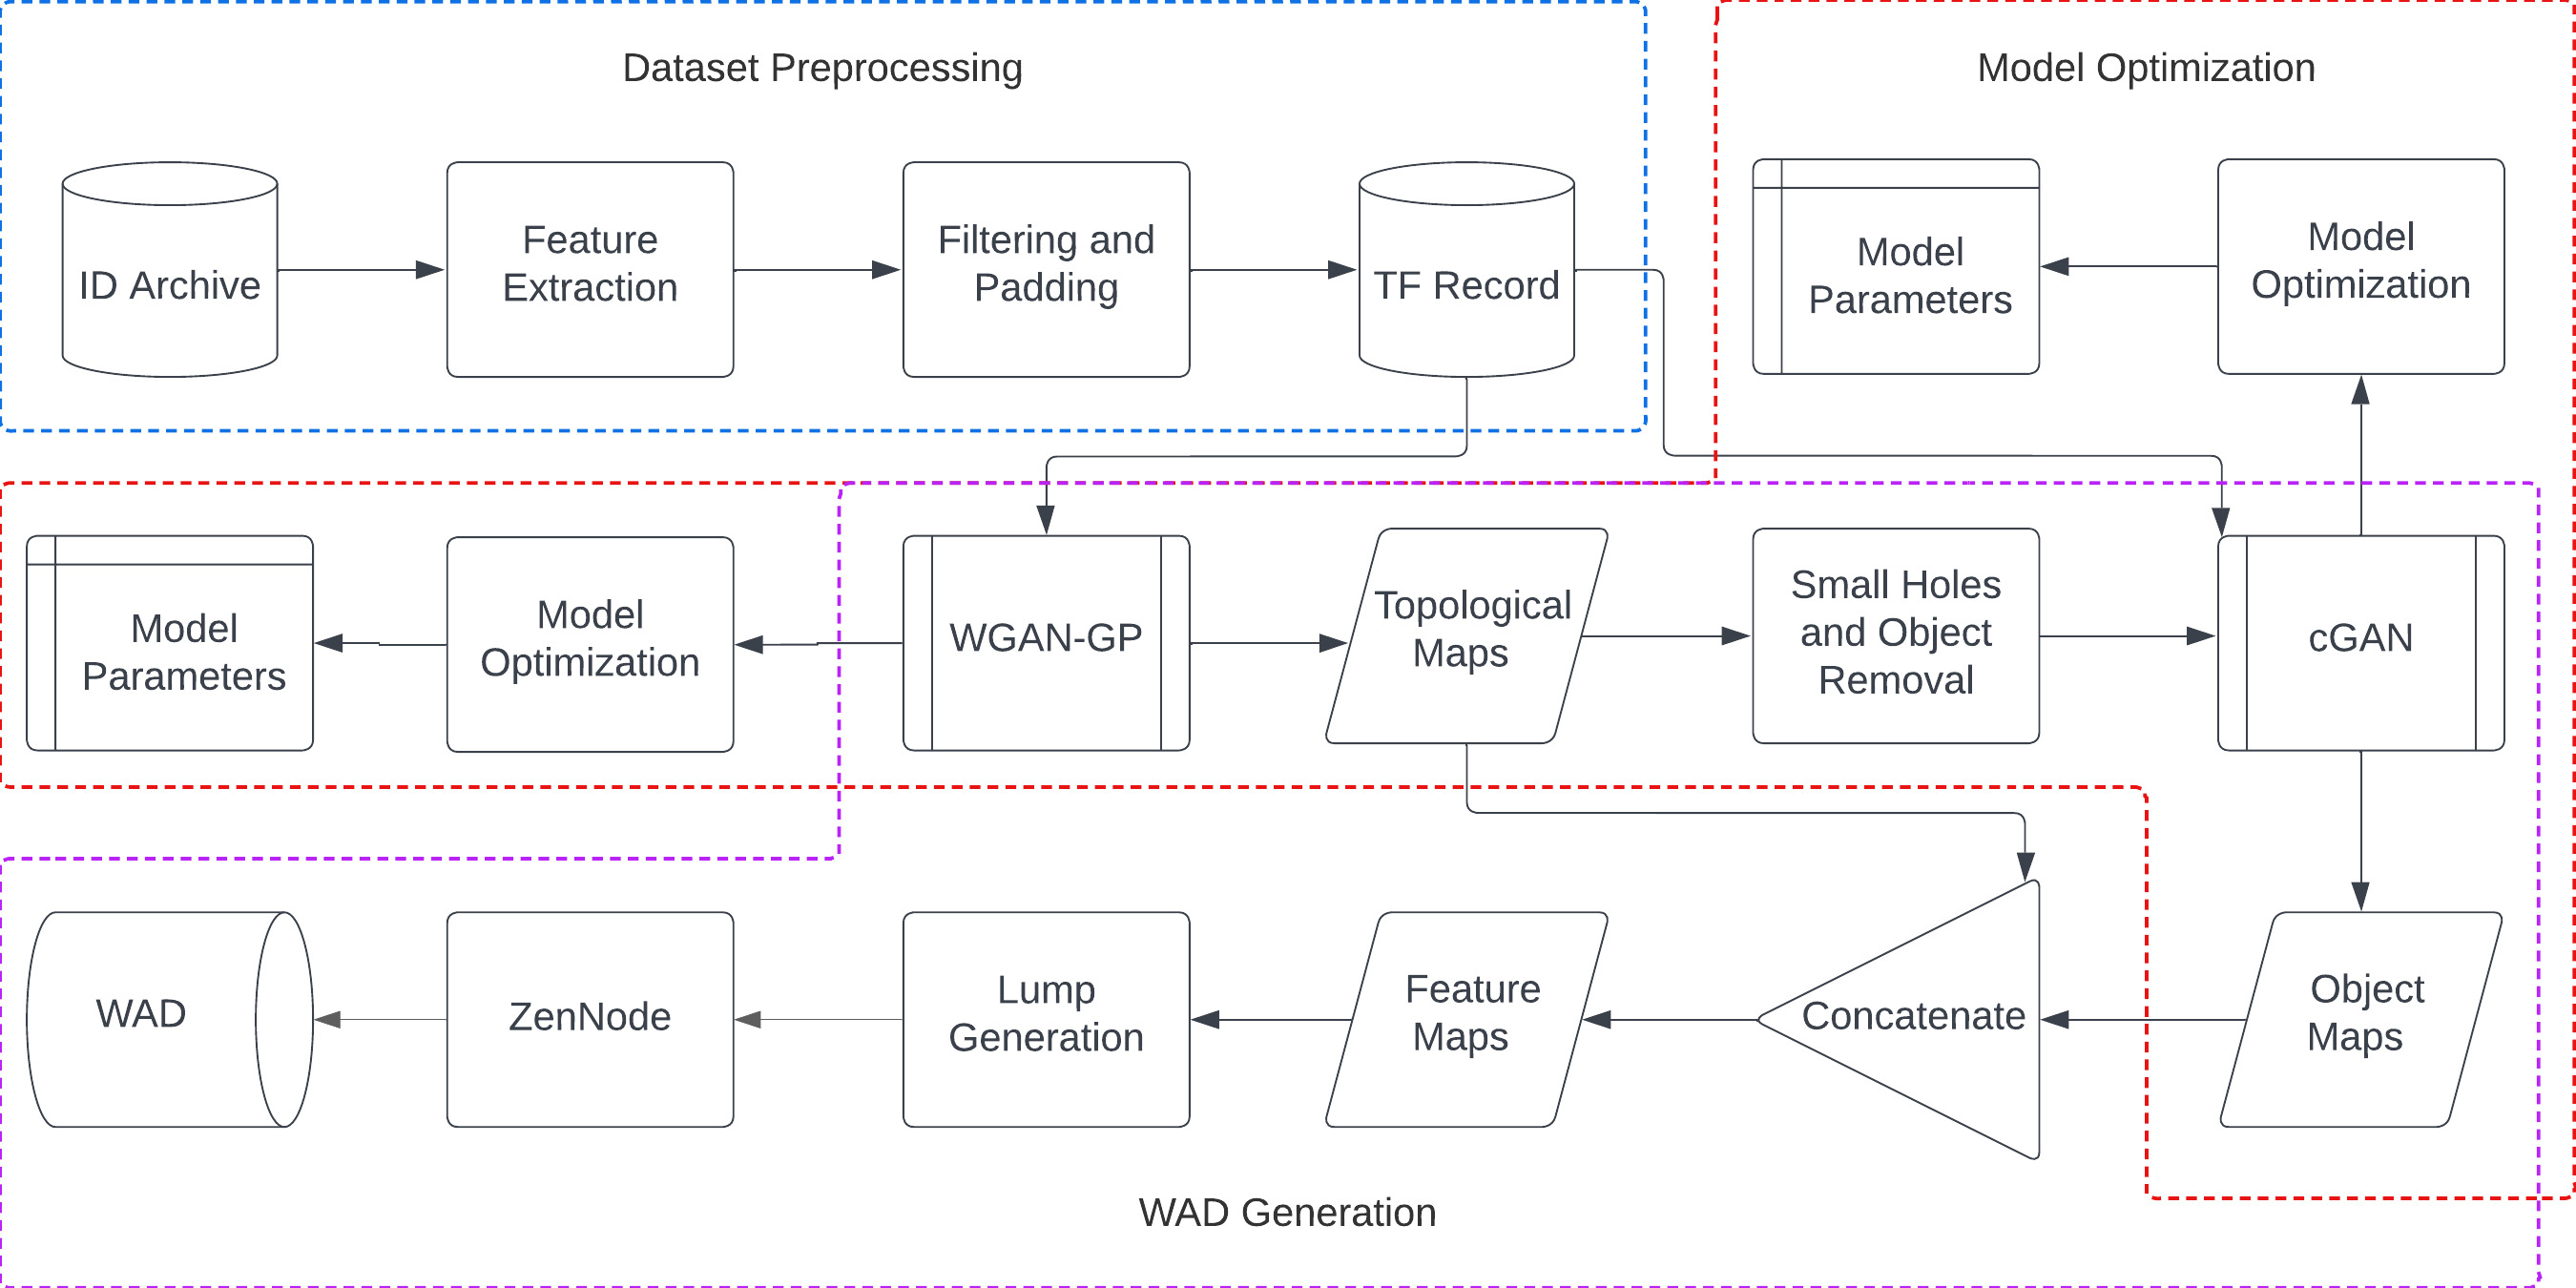
\includegraphics[width=1\textwidth]{data_flow.jpeg}
    \caption{Data flow diagram}
    \label{fig:dataflow}
\end{figure}
The flow of data varies between the two use cases that are being performed by the system. The training case is 
broken into 2 steps, the first of which is the dataset processing phase which begins with the dataset procurement 
of level repository from the archives that appears in the top left of Figure~\ref{fig:dataflow} to obtain the dataset 
as TFRecords. Once the dataset is procured, the model optimization phase uses the dataset until the constructed 
models have been sufficiently taught to obtain the feature maps in a manner that can mimic the dataset.

The next case consists of the generation phase, during which the models transform random 
noise into feature maps with the WGAN-GP’s outputs go through a post processing 
phase to help clear noise and artifacts. The resultant maps are then validated to 
ensure the absence of anomalies before being supplied to the cGAN. Then the model 
outputs are tested through evaluation metrics to inform of its quality and converted 
into WADs for examination of possible in gameplay.
\newpage

\section{Model Optimization}
\subsection{Modified Loss Function}
While the WGAN-GP uses the loss function defined in Section \ref{wgan-gp}, the cGAN network 
performs inconsistently with the $L1$ loss on different optimization attempts from the random 
shuffling of the training dataset. Thus, a suitable loss function has been hand crafted for the 
problem which moves away from the $L1$ loss by replacing it with more milder constraints. 
The first of which is the mask loss $L_{M}$ which is used to compute the number of objects 
that deviate from the bounds of the level. 
\begin{equation} \label{eq:maskloss}
L_{M} = ln|1+\sum_{i=1}^n \sum_{j=1}^n b_{ij} \cdot B(X_{T\char`_Gen_{ij}})|
\end{equation}
Where $b$ indicates if pixel $ij$ is not within the level bounds and $B$ is the binary of the 
presence of a game object at that pixel of the generated maps. The other 
is the object loss $L_{o}$ which is used to approximate the deviation  of the generated objects from 
the true proportions of the categories in that of the true target maps of the level. It is obtained 
through finding the absolute sum error $\epsilon_{as}$ of the generated feature maps from 
that of the target feature maps for each category $k$.
\begin{equation} \label{eq:ase}
\epsilon_{as^k} = |\sum_{i=1}^n \sum_{j=1}^n X_{T\char`_True_{ij}^k} - X_{T\char`_Gen_{ij}^k}|
\end{equation}
\begin{equation} \label{eq:objectloss}
L_{O} = \dfrac{1}{|K|}\sum_{k=1}^K\lambda \cdot ln|1+ \dfrac{\epsilon_{as^k}}{1+ \sum_{i=1}^n \sum_{j=1}^nX_{T\char`_True_{ij}^k}}|
\end{equation}
This error is taken in proportion to the number of target objects to ensure that the categories 
with fewer objects do not get ignored. Just as the mask loss, a natural log is used to modulate  
large loss values towards a more moderate scaling with $\lambda$ amplify its significance. 
Finally, the mean of this loss is taken across the available categories $K$ is then summed with 
the GAN loss from Equation~\ref{eq:patchloss} and the mask loss to derive the total generator’s loss.
\begin{equation} \label{eq:genloss}
L_{G}=-\mathop{{}\mathbb{E}}_{x,z}[log(D(X_{I\char`_True},X_{T\char`_Gen})] + L_{M} + L_{O}
\end{equation}

\subsection{Training Algorithm}
The system is trained through iteratively executing the training operations over 1023
training samples $X_{train}$ with the models validated over the remaining 256 samples 
$X_{Val}$. At the end of each epoch, reference samples are computed using the same 
seed of gaussian noise with a mean of 0 and standard deviation of 1. These are used to 
provide a visual understanding as to the development of the model over the training cycle. 
As the architecture is composed of two separate models, the training algorithm has been 
distinctly tabulated with one detailing the processes performed by the WGAN-GP networks and 
another for the cGAN networks.

This dataset has been artificially enlarged for the WGAN-GP networks to 8064 and 2048 
for training and validation respectively through the consideration of the three 
90-degree rotations and its mirror images to exploit for the differences in level 
orientation. Each of the WGAN-GP networks has been trained for 
100 epochs using a batch size of 16 with validation performed every 100 batches. 
The critic is trained for 3 steps for every step that the generator is trained instead of the 
suggested 5 but performs similarly when compared. A weight of 10 is multiplied to the 
gradient penalty for the critic loss. Both networks utilize Adam optimizers with a learning 
rate of 2e-4, beta decay of 0.5 and momentum set at 0.999.
\begin{table}[H]
\centering 
\begin{tabular}{ |C{2.5cm}|C{2.5cm}|C{2.5cm}|C{2.5cm}|C{2.5cm}|}
\hline
\textbf{Process} & \textbf{Inputs} & \textbf{Outputs} & \textbf{Periodicity} & \textbf{Evaluated Opertors} \\
\hline
Train G & $Z_{U}[0,1]$ & $L_{G\char`_Train}$ & 3 & $X_{Gen}$, $Y_{Gen}$\\
\hline
Train C & $X_{Train}$, $Z_{U}[0,1]$ & $L_{C\char`_Train}$ & 1 & $X_{Gen}$, $Y_{Gen}$, $Y_{Train}$\\
\hline
Validation & $X_{Val}$, $Z_{U}[0,1]$ & $L_{G\char`_Val}$, $L_{C\char`_Val}$ & 300 & $X_{Gen}$, $Y_{Gen}$, $Y_{Val}$\\
\hline
Reference Sample & $Z_{Ref}$ & $X_{G\char`_Ref}$ & 1512 & -\\
\hline
Network Checkpoint & $G$, $G_{Optim}$ & checkpoint & 1512 & -\\
\hline
\end{tabular}
\\[10pt]
\caption{Training operation of WGAN-GP models}
\label{table:wgantrain}
\end{table}
\newpage

The hybrid network on the other hand does not have its dataset enlarged since they 
are trained with a batch size of 1 as consecutive samples with altered orientations 
causes it to retain unnecessary bias when presented with unusual samples from the 
dataset. It is also trained similarly to the WGAN-GP, using the same hyperparameters 
with the exception being that the Adam optimizer has a learning rate of 6e-5 to reduce 
the impact of each batch and avoid reaching a local minimum and a weight of 10 for the object loss.
\begin{table}[H]
\centering 
\begin{tabular}{ |C{2.5cm}|C{2.5cm}|C{2.5cm}|C{2.5cm}|C{2.5cm}|}
\hline
\textbf{Process} & \textbf{Inputs} & \textbf{Outputs} & \textbf{Periodicity} & \textbf{Evaluated Opertors} \\
\hline
Train G & $X_{I\char`_Train}$, $Z_{U}[0,1]$ & $L_{G\char`_Train}$ & 3 & $X_{T\char`_Gen}$, $Y_{Gen}$\\
\hline
Train C & $X_{Train}$, $Z_{U}[0,1]$ & $L_{D_Train}$ & 1 & $X_{T\char`_Gen}$, $Y_{Gen}$, $Y_{Train}$\\
\hline
Validation & $X_{I\char`_Val}$, $X_{T\char`_Val}$, $Z_{U}[0,1]$ & $L_{G\char`_Val}$, $L_{D\char`_Val}$ & 100 & $X_{T\char`_Gen}$, $Y_{Gen}$, $Y_{Val}$\\
\hline
Metrics & $X_{I\char`_Val}$, $X_{T\char`_Gen}$ & $metric_{eval}$ & 100 & -\\
\hline
Reference Sample & $X_{I\char`_ref}$, $Z_{Ref}$ & $X_{G\char`_Ref}$ & 1023 & -\\
\hline
Network Checkpoint & $G$, $G_{Optim}$ & checkpoint & 1023 & -\\
\hline
\end{tabular}
\\[10pt]
\caption{Training operation of cGAN models}
\label{table:cgantrain}
\end{table}

\subsection{Updated WAD Generator}
Feature maps are reverse engineered into the mandatory lumps necessary for
the DOOM engine with the help of certain refinements made to Giacomello’s WAD 
Editor. Firstly, detached regions of the level have been addressed through the 
introduction of post processing before generation of category maps. It removes holes 
and small objects from the floor map to ensure that it is fully connected before 
generating the corresponding category maps. Another issue is the presence of inaccessible 
paths that are caused by narrow corridors between the sections. This happens when the scale 
size of pixel wide sectors is smaller than the player. It has been tackled by ensuring that 
the minimum width of paths represented by pixel is greater than the dimensions of the character 
by enforcing a scaling factor of 128 while never exceeding the bounds of the available level space.

The Doom Engine also uses a Binary Space Partitioning Algorithm for pre-computing 
the Hidden Surface Determination or occlusion culling. In this work, the 
tool ZenNode \cite{MaR04} has been used in the last stage of the pipeline, to produce playable 
DOOM levels from the network output. ZenNode is a 3rd party software used to 
generate lumps that does not directly affect the level design. It has additional 
functionalities with a customizable Binary Space Partition to ignore certain 
lindefs and specify unique sectors, though its main function is to provide 
incomplete PWADs with blockmap and reject resources automatically, given 
that the remainder of the lumps have already been generated using the feature maps.

\subsection{Experimental Setup}
The experiment performed is a comparative analysis between the proposed and prior 
architectures with the traditional model added in to provide plausible justification for 
the added modifications to the hybrid network. While training 
the networks, similar models have been constructed near indistinguishable to 
minimize any variations that are not due to the inherent differences between the 
models. To this end, the networks use the same number of layers, hyperparameters, 
kernel size and stride wherever possible. 

The experiment is set up initially to compare the cGAN networks through metrics 
calculated during the training phase. Although it may seem tempting to simplify the 
functional generator by means of using just a U-Net architecture which only implements the 
object and mask loss as discussed in the previous section, it is incapable of mimicking 
the subtle variations of object placements through performing the image-to-image 
translation purely with a fixed loss function and hence has been rejected for this system.

The traditional WGAN-GP network is not taken into account for the training metrics as it does not 
use a two-step process making it difficult to calculate them without context. It also 
does not use the aforementioned category maps due to its generator’s tendency 
towards producing predominantly zeros matrices for those features due to the sparse 
nature of the distribution. This architecture is found to at least be able to generate 
some game objects when trained with the thingsmap which has been 
included in the post training evaluation of the networks. Post training evaluation is 
done over 100 samples from the real and generated datasets.

\begin{table}[H]
\centering 
\begin{tabular}{ |C{2cm}|C{2.5cm}|C{3.5cm}|C{2.5cm}|C{2.5cm}| }
\hline
\textbf{Model} & \textbf{$G_{Loss}$ Function} & \textbf{Feature Maps} & \textbf{$G$ Convolutional Layers (filters)} & \textbf{$D$ Convolutional Layers (filters)} \\
\hline
WGAN-GP & Wasserstien Distance with Gradient Penality & floormap, heightmap, wallmap, thingsmap & 4 (1024, 512, 256, 128) & 4 (128, 256, 512, 1024)\\
\hline
\multirow{2}{4.5em}{\centering WGAN-GP + Tradition cGAN} & Wasserstien Distance with Gradient Penality & floormap, heightmap, wallmap &  4 (1024, 512, 256, 128) & 4 (128, 256, 512, 1024)\\ \cline{2-5}
 & Cross Entropy + $L1$ Norm & monstersmap, ammunitionsmap, powerupsmap, artifactsmap, weaponsmap & 7 (128, 256, 512, 1024, 1024, 512, 256) & 4 (128, 256, 512, 1024)\\ 
\hline
\multirow{2}{4.5em}{\centering WGAN-GP + Modified cGAN} & Wasserstien Distance with Gradient Penality & floormap, heightmap, wallmap &  4 (1024, 512, 256, 128) & 4 (128, 256, 512, 1024)\\ \cline{2-5}
 & Cross Entropy + Object Loss + Mask Loss & monstersmap, ammunitionsmap, powerupsmap, artifactsmap, weaponsmap & 7 (128, 256, 512, 1024, 1024, 512, 256) & 4 (128, 256, 512, 1024)\\ 
\hline
\end{tabular}
\\[10pt]
\caption{Trained architectures used for the comparative study}
\label{table:trainednetworks}
\end{table}


\chapter{Results}
\label{ch:results}%

\section{Evaluation Metrics}
The focus of this portion of the thesis is to quantify the evaluations that have 
been made through the results obtained from the experiments using the proposed 
metrics. The preliminary analysis is done to provide plausible justification for the use of the 
modified cGAN network through the training metrics that have been acquired 
alongside its validation by showcasing their differences. The metrics consist of the 
discriminator’s ability to classify the levels, the unique information needed to 
describe the level as well as the following statistics:
\begin{itemize}
\item Mean Object Count – It is the count of all objects within a level by the total 
area that the level occupies. It provides an approximate object density that is 
found in levels and serves as a constraint to check if the object maps are 
leaning towards over saturation or under saturation as the model must learn 
to balance increasing the availability of objects while avoiding overpopulating
a level by making it too congested.
\item Mean Encoding Error – The network generates images where pixels are encoded 
using continuous values which can be rounded towards the closest object type. As the 
networks use a ReLU activation function in the output layer due to the tendency of the 
cGANs towards predominately empty images with sigmoid activation, there is the ability 
to encode values  beyond the limits of assigned ids of the respective categories. This 
error is used to measure the inaccuracy in pixel values which would overflow into other 
categories if not addressed.
\item Mean Out of bounds Error – When objects are generated outside the bounds 
of the level, they are ignored in the level generation process as they are 
inherently inaccessible to the player and thus not part of the actual level. This 
error is used to quantify how often this occurs and the degree to which the 
network is unable to comprehend the constraints within which game objects 
need to be placed.
\end{itemize}
\newpage

It is difficult to compute the former metrics during the training of the traditional WGAN-GP 
since it is learning the complete distribution and they require a definitive level structure 
which is not yet established, making it impractical to compare their respective graphs. 
Instead a set of post training metrics are used to provide a more appropriate analysis. 
These include the performance of the generator in understanding the problem by 
identifying visual artifacts in the presentation of the things map and distinguishing 
the samples intuitively. as well as the analyzing the object distribution, both spatially 
and categorically. While not it is not completely comprehensive,  it should provide conclusive 
evidence of their abilities. These later techniques assess the presence of a game object around 
the surrounding context, be it the local section or the encompassing level and are 
described as follows:
\begin{itemize}
\item Proportions Analysis – It is based on the proportions of the various categories 
based on the types of objects that it uses to populate the level. This is used to 
understand how well the model is able to grasp the relation between the 
requirement of placing objects from different categories and significance of 
their individual types. This in junction with the count of the individual object 
type from the available categories provide a clear picture on the biases and 
tendencies of the generator when applying a positive encoding on any pixel.
\item RipleyK Function – It is used to measure the spatial distribution of the generated 
objects \cite{BdR17}. It determines whether points have a random, dispersed, or 
clustered distribution pattern. The function is calculated by taking the average
 occurrence of events within a predetermined radius of every point iteratively 
which provides an advantage over other methods since it is independent of the density
 of the point pattern and thus can describe the spatial point patterns at many different 
scales \cite{LiW15}. The function is evaluated as follows:
\begin{equation} \label{eq:ripleyk}
K(s) = \lambda^{-1} n^{-1} \sum_{i=1}^n \sum_{j\neq 1} I(d_{ij}<s)
\end{equation}
where $d_{ij}$ represents the distance between points $i$ and $j$, $s$ is the threshold 
radius within which the point is considered and $n$ is the number of points 
that are sampled from the distribution with $\lambda$ being the reduction factor 
of the function. 
\end{itemize}
\newpage

\section{Model Evaluation}
\subsection{Training Metrics}
By using the loss computed during the training sequence, we are able to compare the 
variation in the discriminator's ability to identify the generated levels. As both cGANs 
use different loss functions in their generators, it is difficult to directly
compare their assessments and thus more emphasis will be given between graphs of 
the discriminators from both models of the hybrid architecture. Although 
validation data is not as useful in GANs to assess overfitting and/or implement early 
stopping, it is still done to hold back some real samples for testing the discriminating 
network to compare how well it can classify images among the functional generators 
\cite{DeT20}. This can be seen in Figure~\ref{fig:tradloss} with the discriminator validation
 loss of the traditional cGAN rising above that of its training counterpart around the 40th 
epoch while the network is only able to generate viable samples after the 80th epoch.
\begin{figure}[H]
    \centering
    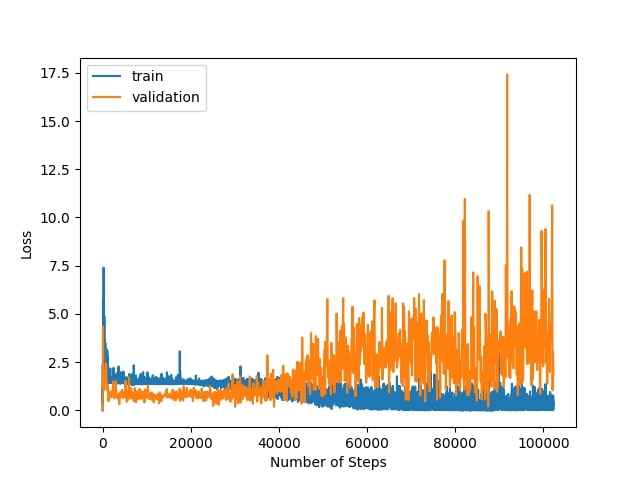
\includegraphics[width=0.9\textwidth]{trad_cgan_loss.jpg}
    \caption{Discriminator Loss of the traditional cGAN model}
    \label{fig:tradloss}
\end{figure}
\begin{figure}[H]
    \centering
    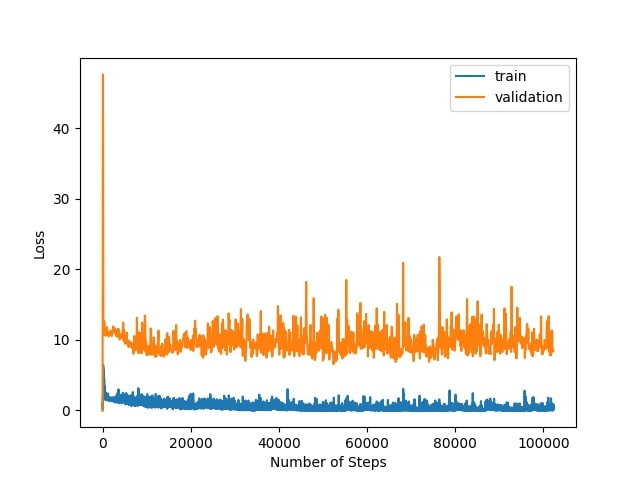
\includegraphics[width=0.9\textwidth]{mod_cgan_loss.jpg}
    \caption{Discriminator Loss of the modified cGAN model}
    \label{fig:modloss}
\end{figure}
As seen in Figure~\ref{fig:tradloss} and Figure~\ref{fig:modloss}, the traditional cGAN is better at deceiving its
discriminator with a smaller loss value but is plagued with inconsistencies due to the 
stricter constraints of the $L1$ norm present in the generator loss when handling 
outliers in the training dataset, leading to a more noisier graph when compared to 
the laxer restrictions imposed by the object and mask loss. This is also seen in the fact 
that the traditional cGAN performs very differently from independent instances of the 
complete training cycle and seems to be extremely sensitive towards the shuffling 
process while the modified cGAN is able to repeatedly settle at a minima that provides 
consistent results.
\begin{figure}[H]
    \centering
    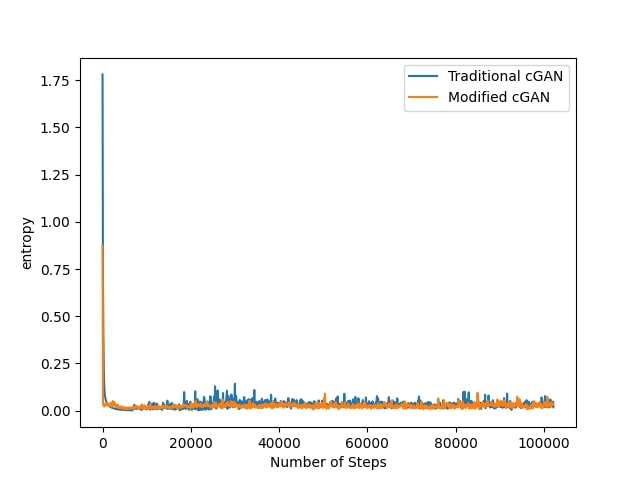
\includegraphics[width=0.85\textwidth]{entropy.jpg}
    \caption{Mean entropy of the generated category maps}
    \label{fig:entropy}
\end{figure}
\begin{figure}[H]
    \centering
    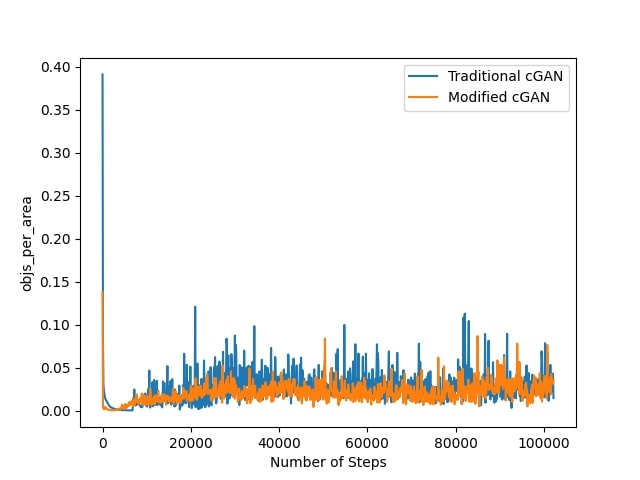
\includegraphics[width=0.85\textwidth]{obj_count.jpg}
    \caption{Mean object count per unit area of the generated category maps}
    \label{fig:objcount}
\end{figure}
Figure~\ref{fig:entropy} and Figure~\ref{fig:objcount} show the similarities between the cGAN networks with amount of 
randomness and the object counts being approximately the same during the training 
process which is misleading when not taken into context with the errors produced by 
the networks. The next set of metrics provide a better understanding of this 
inconsistency of the traditional cGAN with the encoding error showing lesser 
accuracy for assigning values within the limits of the object ids and the out of bounds 
error highlighting the positioning the objects outside the prescribed level space
\begin{figure}[H]
    \centering
    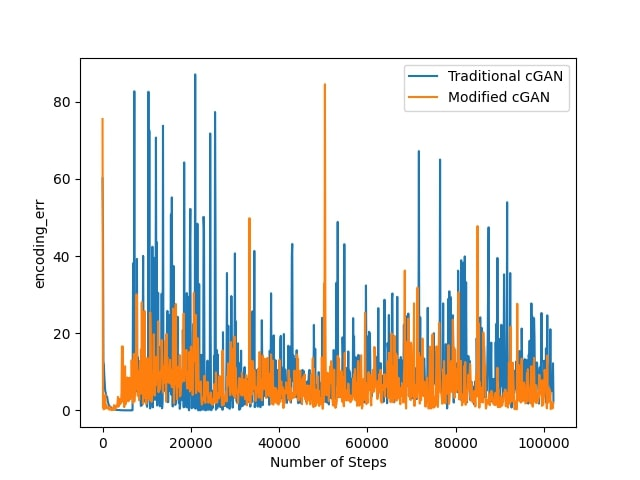
\includegraphics[width=0.9\textwidth]{enc_err.jpg}
    \caption{Mean encoding error of the generated category maps}
    \label{fig:encerror}
\end{figure}
Even though the traditional cGAN provides a object count in line with its modified 
counterpart, most of the objects that have been generated are not within the limit of 
the dictionary ids as seen in Figure~\ref{fig:tradcgansample1} and Figure~\ref{fig:tradcgansample2} 
which has an negative effect to the otherwise normal object count
after the correction is made. This is caused by outliers that occur within the repository of 
feature maps because some custom levels having an unusual distribution such 
as higher count of more significant object types in some categories while the others 
only having a few less significant object types.
\begin{figure}[H]
    \centering
    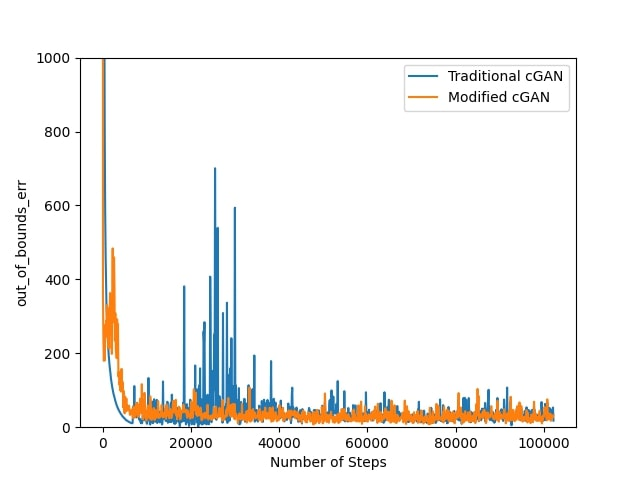
\includegraphics[width=0.9\textwidth]{oob_err.jpg}
    \caption{Mean out of bounds error of the generated category maps}
    \label{fig:ooberror}
\end{figure}
The out of bounds error paints a similar picture with traditional cGAN suffering from 
the inability to generate objects within the predefined levels space consistently and 
this greatly vary among distinct repetitions of the training cycle as the dataset is 
shuffled differently at each instance. In an attempt to rectify, the network 
overcorrects which leads to the sensitivity that is noticed from before. There is also 
other issues that are encountered such as its ability to allot game object type less
evenly among the categories by heavily favouring certain categories during the 
generation process. This is clearly visible in Figure~\ref{fig:categoyproportions} where the favoured category 
keeps varying throughout the multiple independent repetitions of the training algorithm.
\newpage

\subsection{Proportions Analysis}
By separating the problems, the hybrid architecture with a modified cGAN is shown
to better learn the distribution of the various object categories while maintaining 
appropriate object density when compared to the traditional WGAN-GP as well as the 
traditional cGAN. Figure~\ref{fig:categoyproportions} shows the percentage of objects 
belonging to each category from sampled levels. While the overall proportions are 
a major concern in determining the quality of gameplay, there is also a need to 
moderate the intensity created by the individual object based on the type within the 
category. As such boss level monsters or the BFG 3000 require a much more 
appropriate environment to appreciate its presence and must be reflected in the 
number present in each level. In such cases, the modified cGAN adheres to these 
principles and sparingly generates objects of higher significance which can be observed 
in Appendix~\ref{appendixa} that provides average count of each object for every 
category within the levels.
\begin{figure}[H]
    \centering
    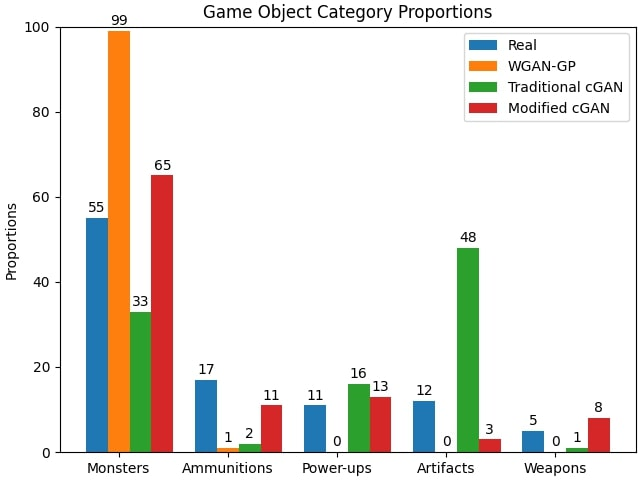
\includegraphics[width=1\textwidth]{cate_props.jpg}
    \caption{Average proportions of each category for sampled levels}
    \label{fig:categoyproportions}
\end{figure}
\newpage

\subsection{Spatial Homogeneity}
The Ripley-K results are interpreted with larger values being the outcome of distributions that 
have greater deviation to completely spatial random distributions or are not spread 
homogenously across the given space. Table~\ref{table:ripleykavg} records the average spread of the 
objects with the results closest to the real distribution being that of the Modified cGAN architecture. 
It is measured at various radii with the histograms of all of the networks at each radius provided in Appendix~\ref{appendixb}. 
This is done as points have a greater tendency to cluster or spread when focusing on larger or 
smaller portions than compared to the actual size of the normalized maps \cite{JoS18}.
\begin{table}[H]
\centering 
\begin{tabular}{ |C{2cm}|C{2.5cm}|C{2.5cm}|C{2.5cm}|C{2.5cm}| }
\hline
\textbf{Radius} & \textbf{Real Distribution} & \multicolumn{1}{c|}{\textbf{WGAN-GP}} & \textbf{Traditional cGAN} & \textbf{Modified cGAN} \\
\hline
0.5 &  0.358682 & 1.044825 & 0.367623 & 0.309959\\
\hline
0.6 & 0.354013 & 1.125575 & 0.353378 & 0.317495\\
\hline
0.7 & 0.349421 & 1.137372 & 0.327674 & 0.308026\\
\hline
0.8 & 0.337955 & 1.098033 & 0.277786 & 0.290994\\
\hline
0.9 & 0.314244 & 1.014245 & 0.217251 & 0.262595\\
\hline
1.0 & 0.276590 & 0.877306 & 0.146254 & 0.218715\\
\hline
\end{tabular}
\\[10pt]
\caption{ Average Ripley K value taken at multiple radii}
\label{table:ripleykavg}
\end{table}
The traditional WGAN-GP network has a greater average Ripley-K result at each of the 
radii due to overly clumping its game objects near the walls its level structure as well 
as enlarging the sample space due to the presence of small objects. This is drastically 
reduced through post processing the topological feature maps as well as using either cGAN 
networks as it provides a more homogeneous distribution which is in line with that shown 
by the results from the real feature maps and is why they both lead to a similar result. 
\newpage

\section{Sample Generation}
\subsection{Traditional WGAN-GP Model}
\begin{figure}[H]
    \centering
    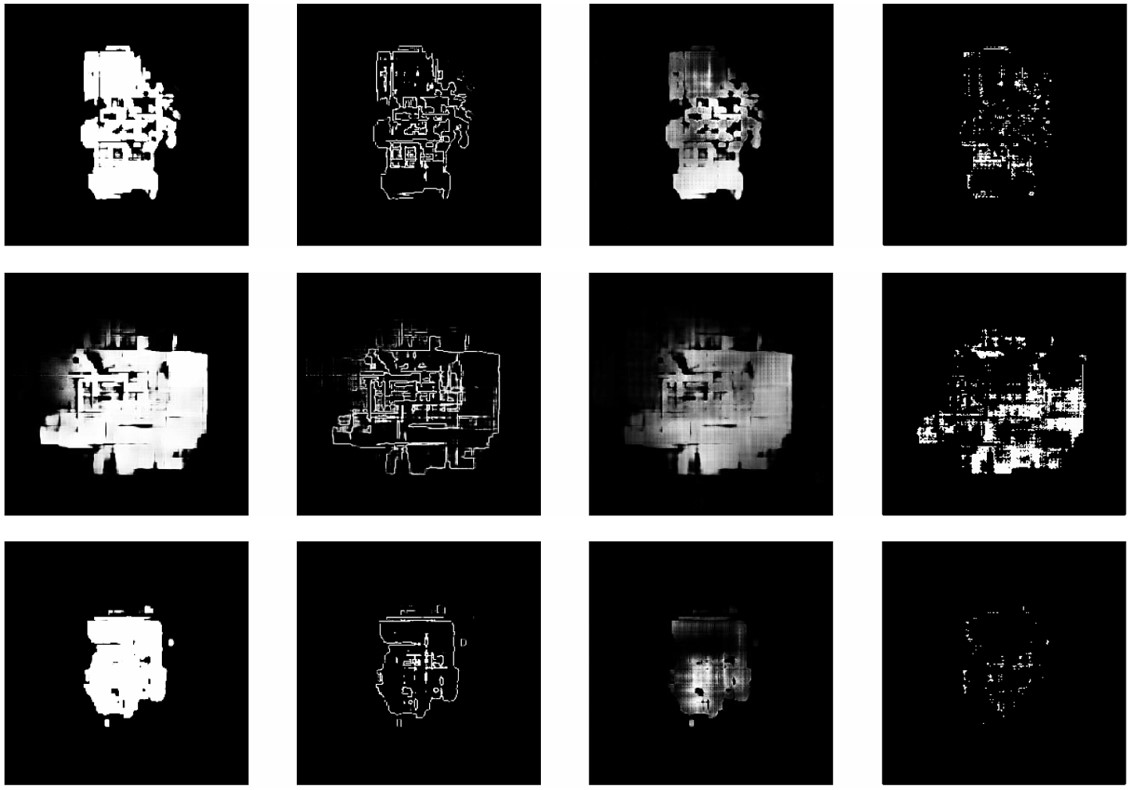
\includegraphics[width=1\textwidth]{wgan_sample.jpg}
    \caption[Samples generated using the traditional WGAN-GP architecture]{Floor map, Height map, Wall map and Things map (columns) generated using the traditional WGAN-GP architecture}
    \label{fig:wgansample}
\end{figure}
As seen in Figure~\ref{fig:wgansample}, the traditional WGAN-GP network  is capable of interpreting 
relations between the wall and floor layouts as well as providing the appropriate height of the 
various sections but is unable to capture the distribution of the various game objects 
across the level due to the increased complexity of the problem. As such there occurs 
a disparity in the distribution of game objects among the categories by mostly 
generating objects for the first category of the sequenced dictionary id with emphasis 
towards lower values shown in Figure~\ref{fig:wgansample1} and Figure~\ref{fig:wgansample2}. 
This is better in comparison to training it with the expanded feature maps as it usually generated zero 
matrices for the categorical features.
\begin{figure}[H]
    \centering
    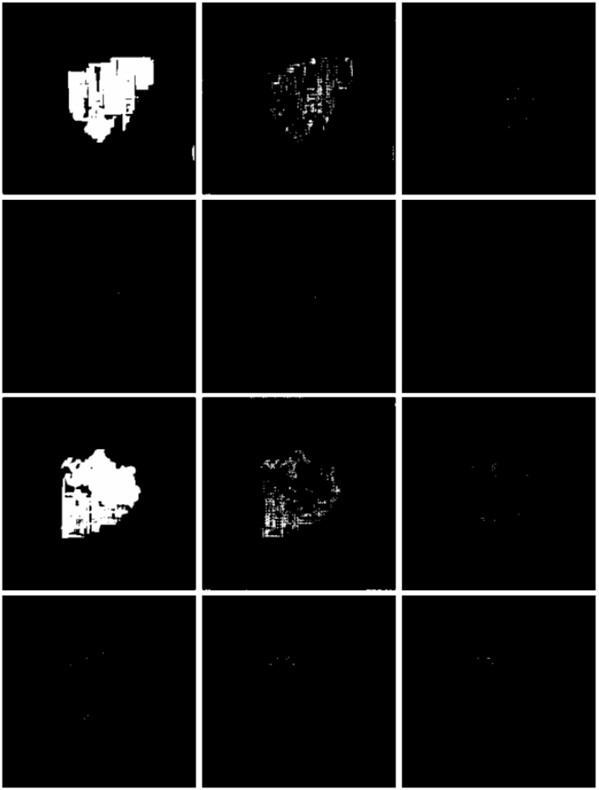
\includegraphics[width=1\textwidth]{wgan_sample1.jpg}
    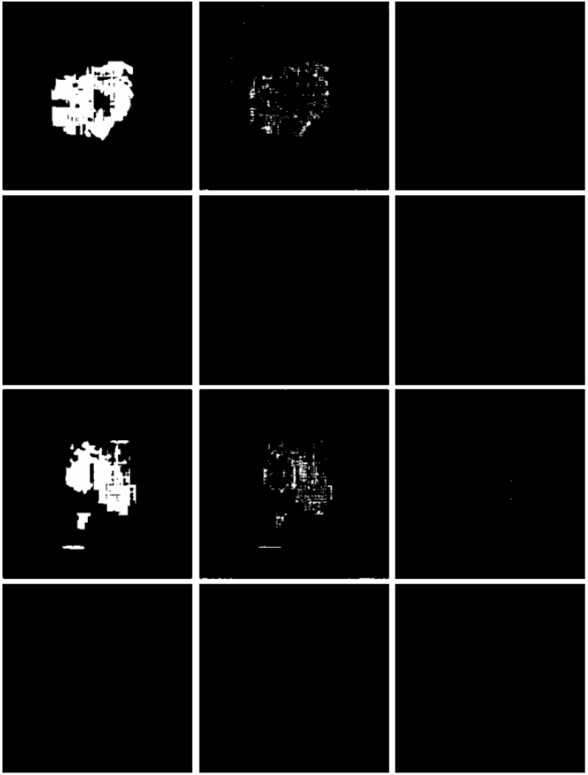
\includegraphics[width=1\textwidth]{wgan_sample2.jpg}
    \caption[Samples generated using the traditional WGAN-GP architecture (1 of 2)]{Floor, Monsters, Ammunitions, Powerups, Artifacts and Weapons Map 
(Column pairs) generated using the traditional WGAN-GP network (1 of 2)}
    \label{fig:wgansample1}
\end{figure}
\begin{figure}[H]
    \centering
    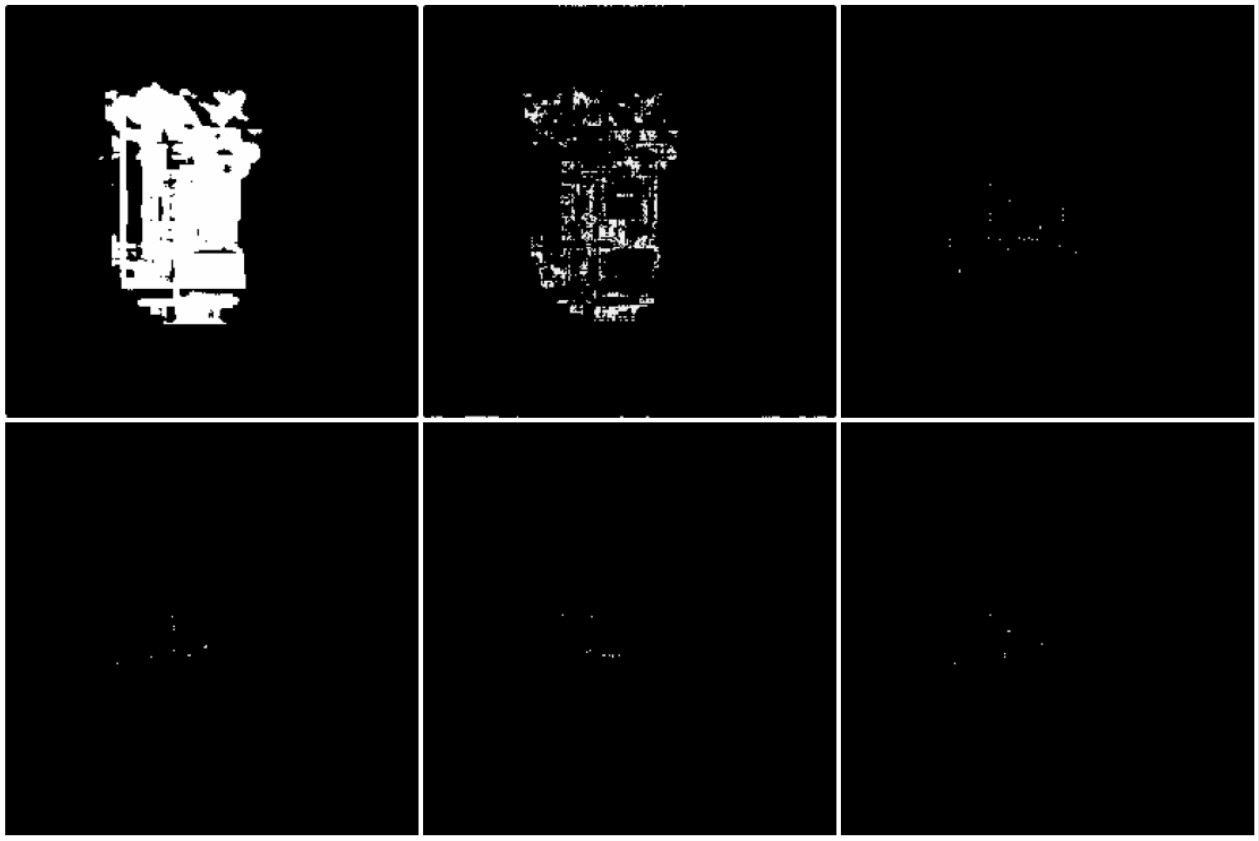
\includegraphics[width=1\textwidth]{wgan_sample3.jpg}
    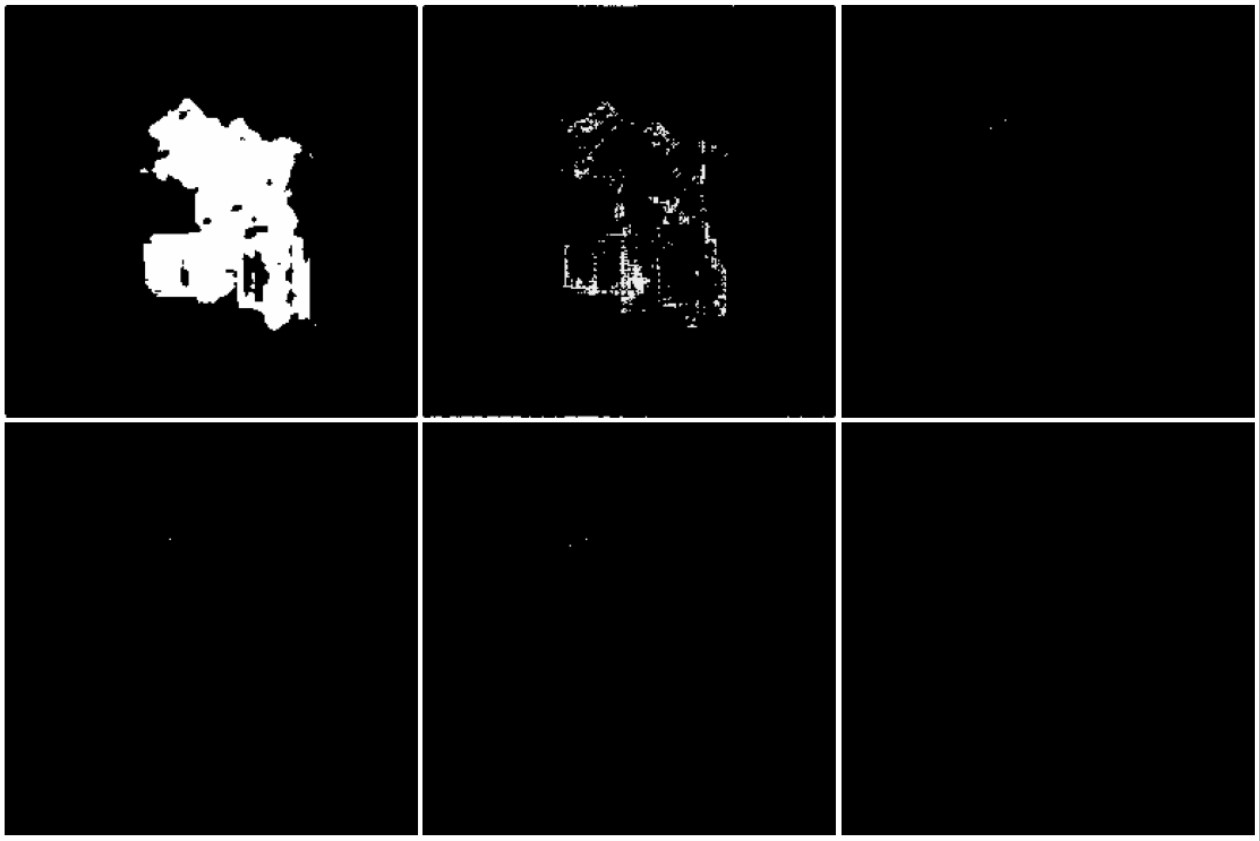
\includegraphics[width=1\textwidth]{wgan_sample4.jpg}
    \caption[Samples generated using the traditional WGAN-GP architecture (2 of 2)]{Floor, Monsters, Ammunitions, Powerups, Artifacts and Weapons Map 
(Column pairs) generated using the traditional WGAN-GP network (2 of 2)}
    \label{fig:wgansample2}
\end{figure}

\subsection{Hybrid Model with Traditional cGAN}
\begin{figure}[H]
    \centering
    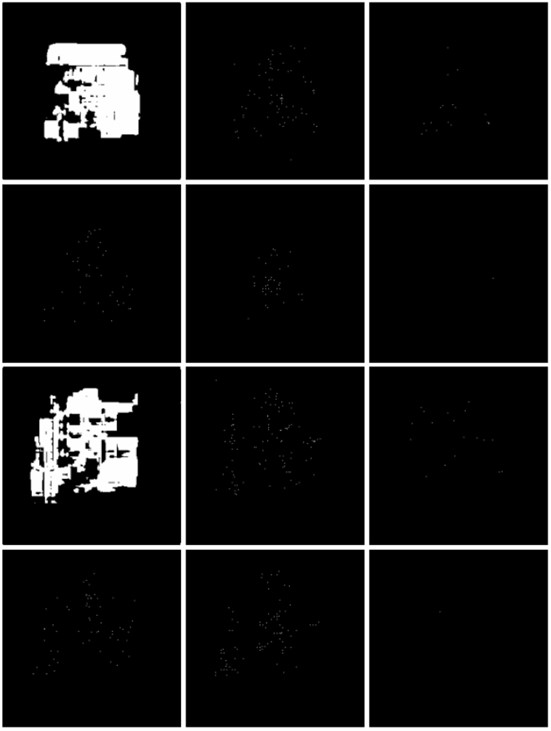
\includegraphics[width=1\textwidth]{trad_cgan_sample1.jpg}
    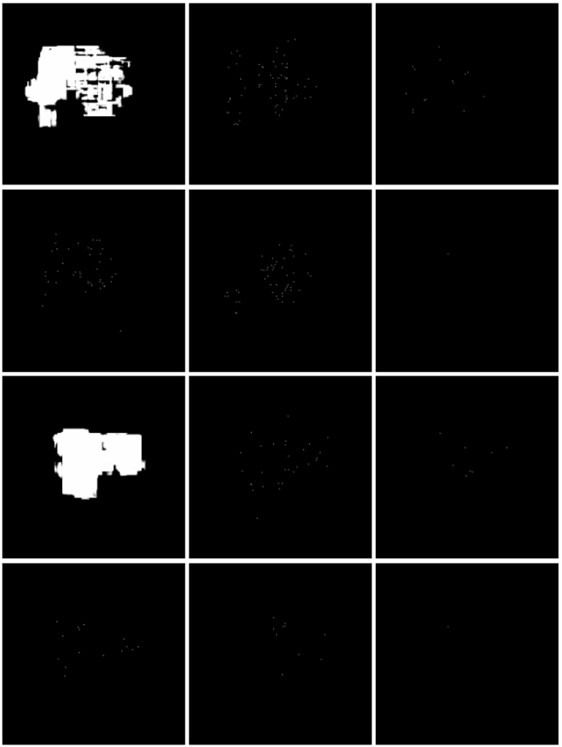
\includegraphics[width=1\textwidth]{trad_cgan_sample2.jpg}
    \caption[Samples generated using the traditional cGAN network (1 of 2)]{Floor, Monsters, Ammunitions, Powerups, Artifacts and Weapons Map 
(Column pairs) generated using the hybrid architecture with traditional cGAN network (1 of 2)}
    \label{fig:tradcgansample1}
\end{figure}
\begin{figure}[H]
    \centering
    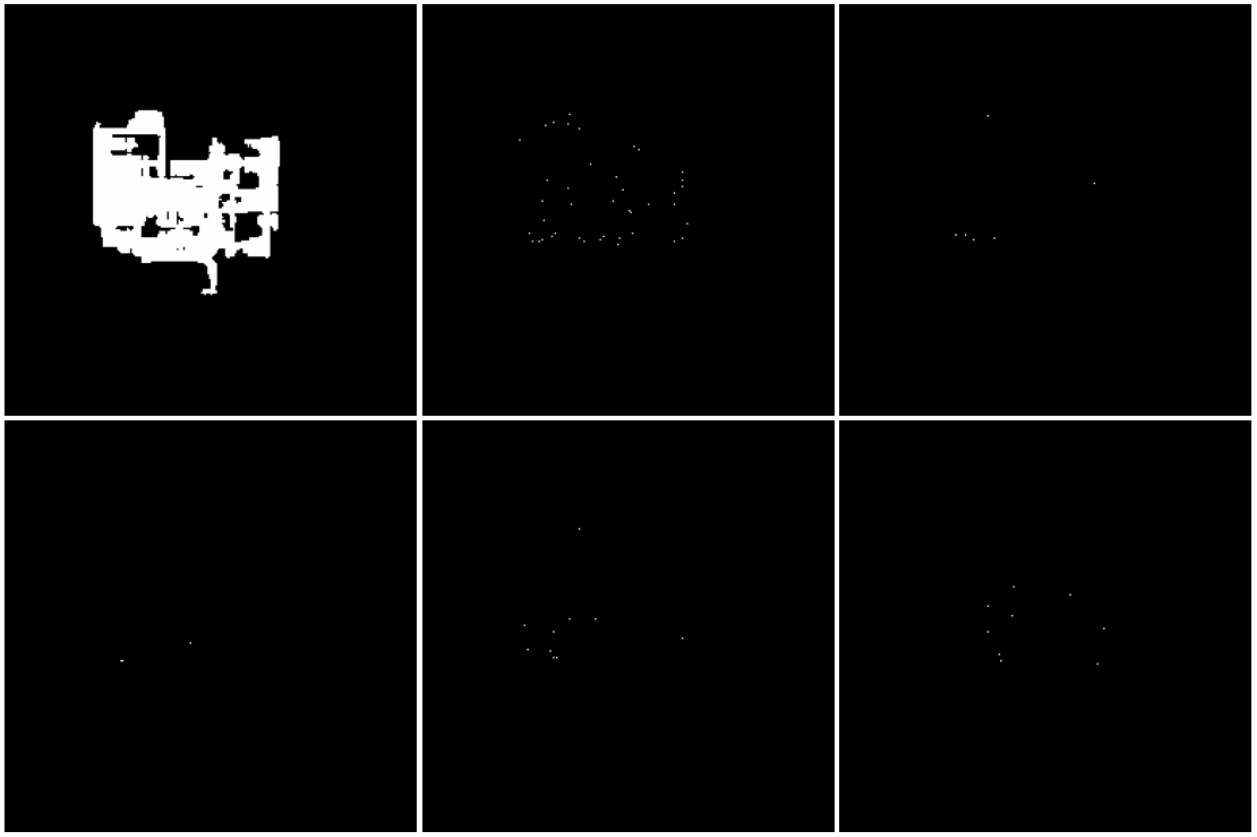
\includegraphics[width=1\textwidth]{trad_cgan_sample3.jpg}
    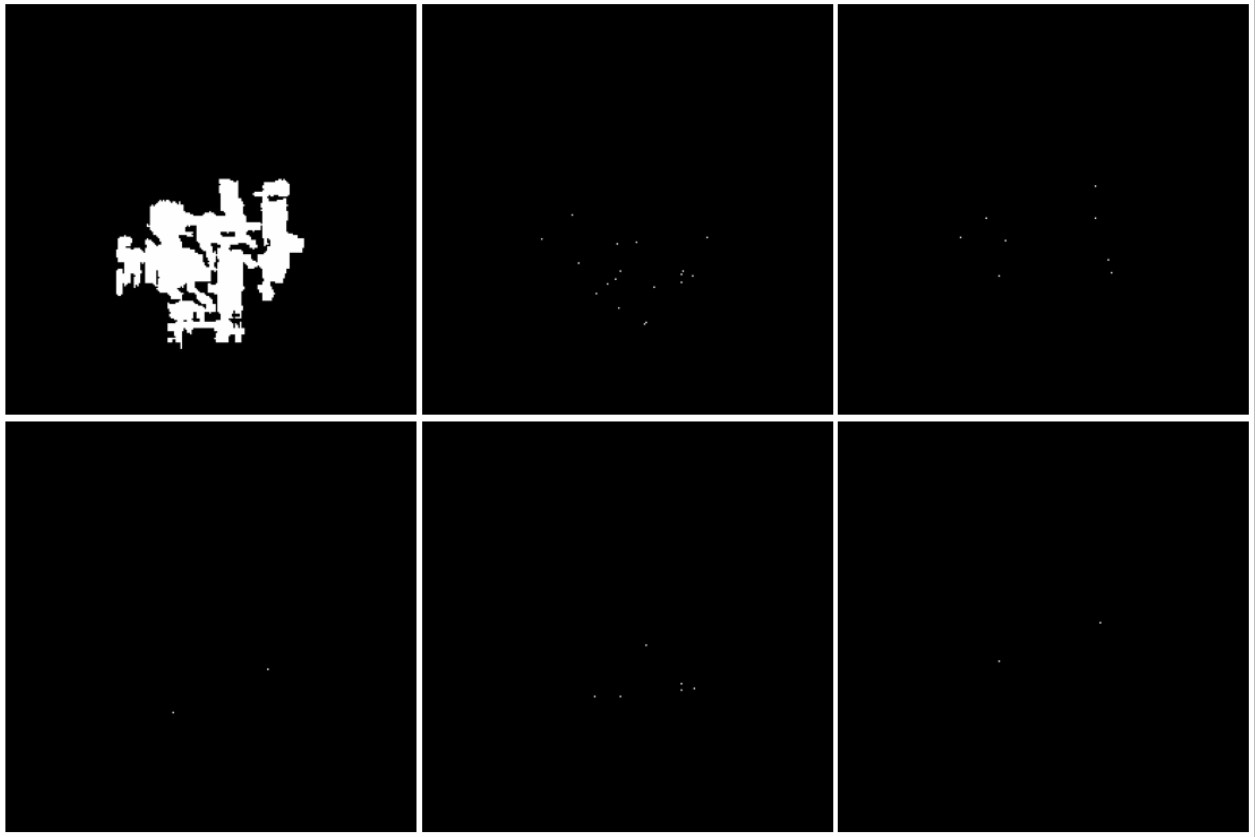
\includegraphics[width=1\textwidth]{trad_cgan_sample4.jpg}
    \caption[Samples generated using the traditional cGAN network (2 of 2)]{Floor, Monsters, Ammunitions, Powerups, Artifacts and Weapons Map 
(Column pairs) generated using the hybrid architecture with traditional cGAN network (2 of 2)}
    \label{fig:tradcgansample2}
\end{figure}

\subsection{Hybrid Model with Modified cGAN}
\begin{figure}[H]
    \centering
    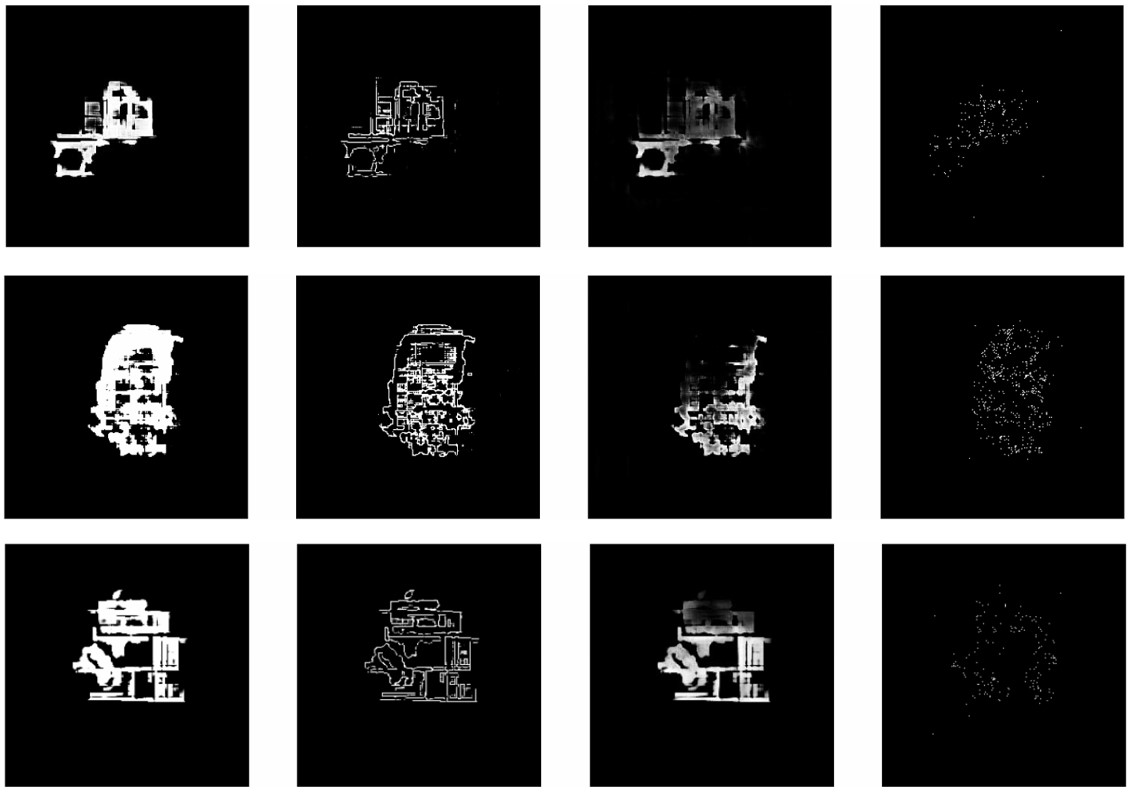
\includegraphics[width=1\textwidth]{mod_cgan_sample.jpg}
    \caption[Samples generated using the modified cGAN network]{Floor map, Height map, Wall map and Things map (rows) generated 
using the hybrid architecture with modified cGAN network}
    \label{fig:modcgansample}
\end{figure}
The hybrid network works around this by separating it into 2 distinct subproblems, 
allowing the WGAN-GP to focus primarily on the level structure while the cGAN
network maps the object positions from the generated level structure. This also 
allows the WGAN-GP to focus more resources towards learning the topological 
distribution which helps in the development of better level layouts to a certain 
extent. This does not ensure that its structure is always better given a random seed as 
the samples that have been use are handpicked to showcase the best results of 
all the trained architectures. As both hybrid models use the same WGAN-GP generator, the 
topological maps are the same with the only difference lying in its generated object 
maps.
\begin{figure}[H]
    \centering
    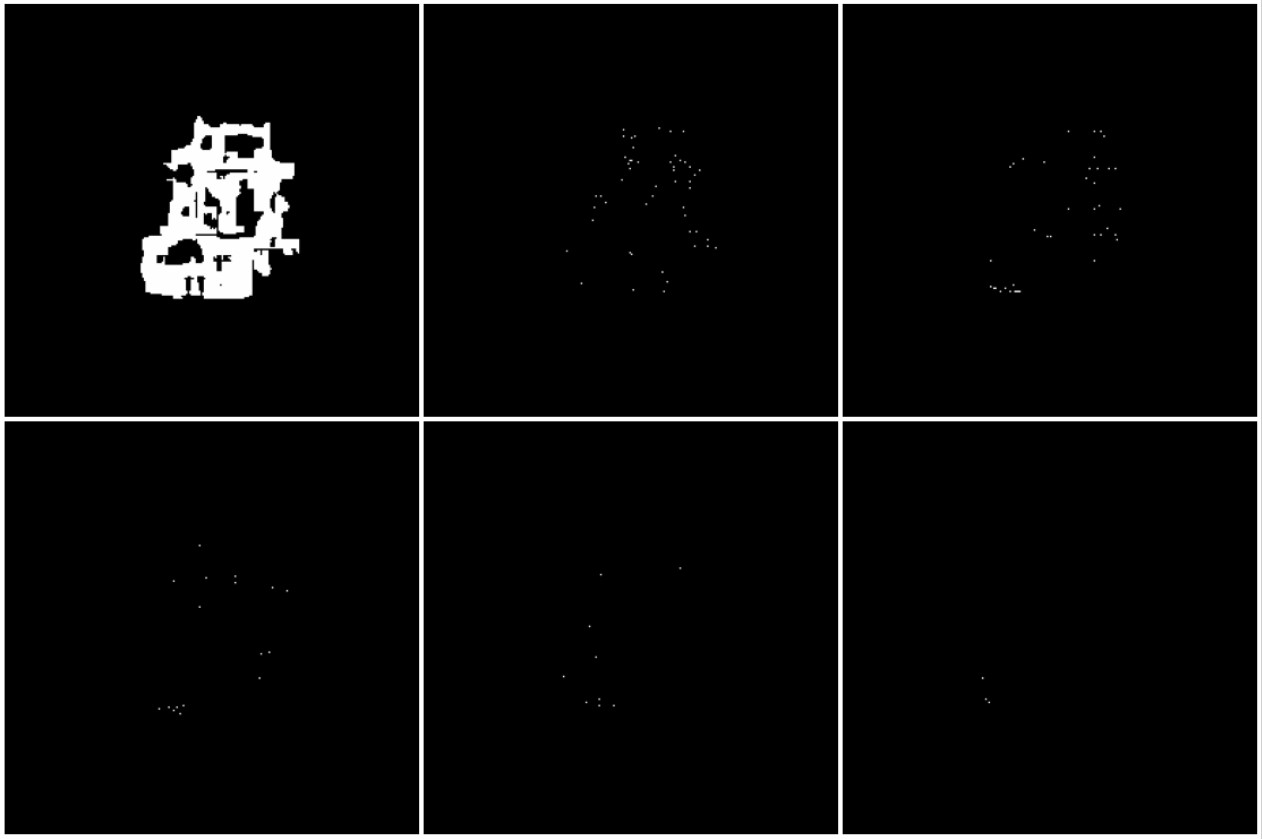
\includegraphics[width=1\textwidth]{mod_cgan_sample1.jpg}
    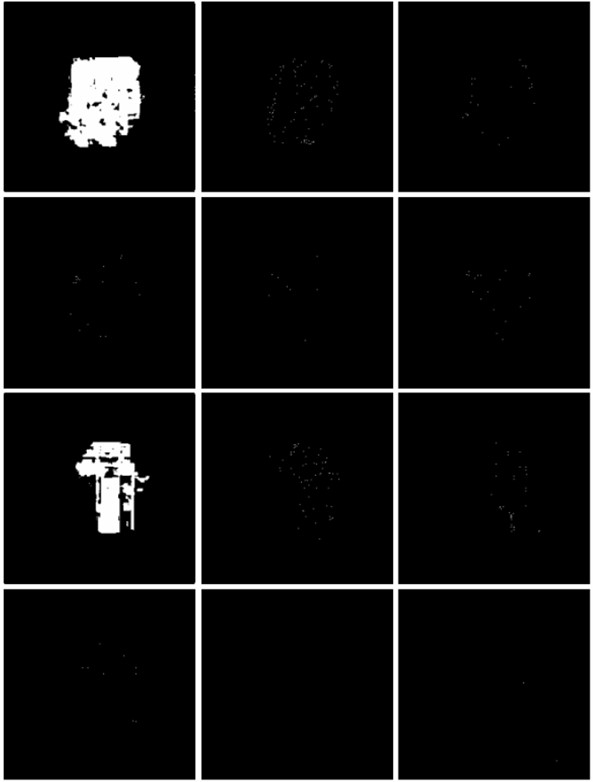
\includegraphics[width=1\textwidth]{mod_cgan_sample2.jpg}
    \caption[Samples generated using the modified cGAN network (1 of 2)]{Floor, Monsters, Ammunitions, Powerups, Artifacts and Weapons Map 
(Column pairs) generated using the hybrid architecture with modified cGAN network (1 of 2)}
    \label{fig:modcgansample1}
\end{figure}
\begin{figure}[H]
    \centering
    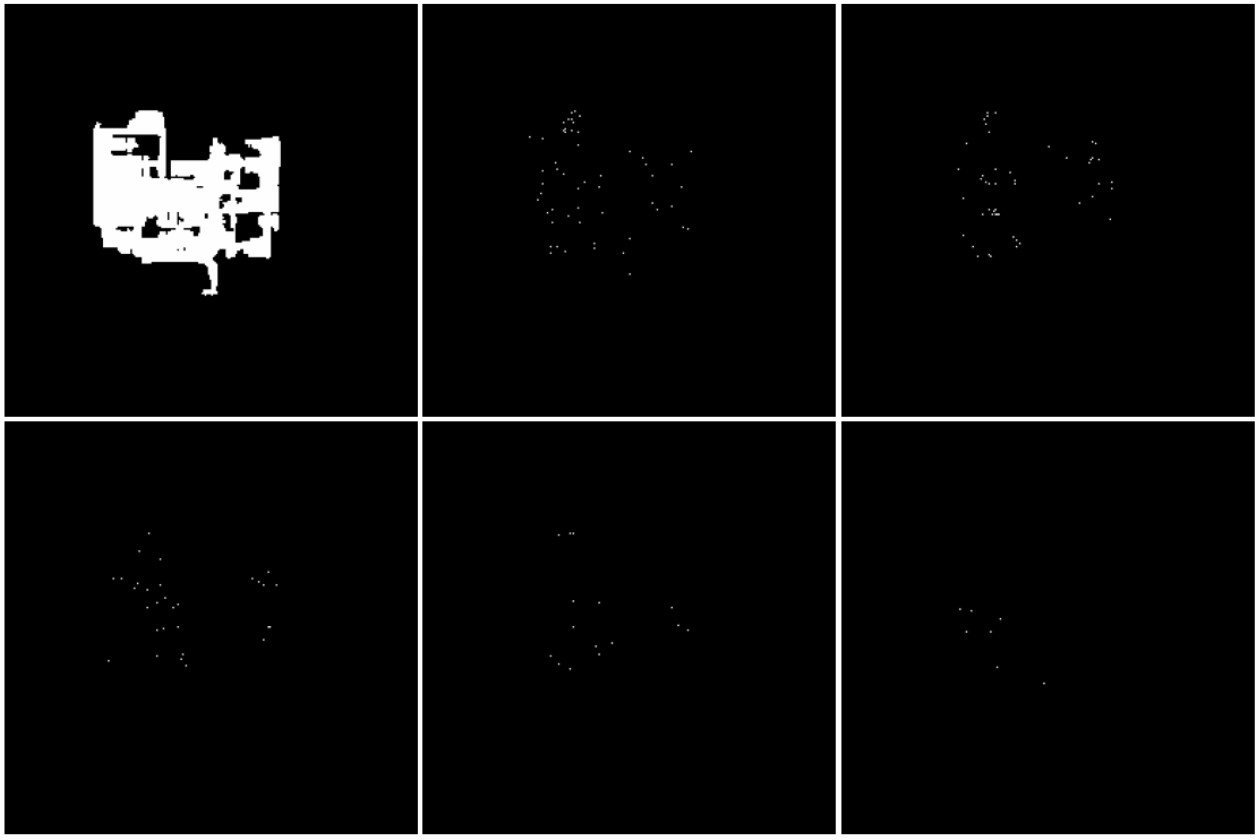
\includegraphics[width=1\textwidth]{mod_cgan_sample3.jpg}
    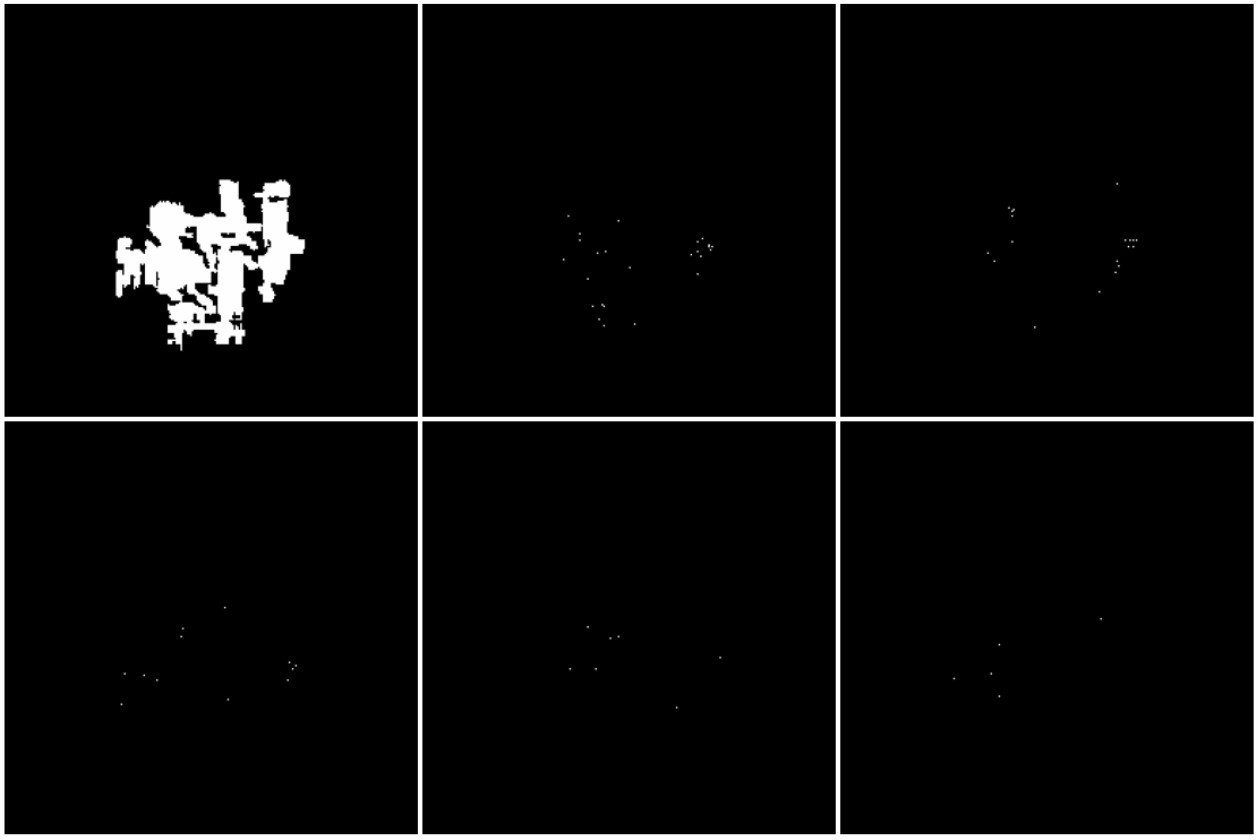
\includegraphics[width=1\textwidth]{mod_cgan_sample4.jpg}
    \caption[Samples generated using the modified cGAN network (2 of 2)]{Floor, Monsters, Ammunitions, Powerups, Artifacts and Weapons Map 
(Column pairs) generated using the hybrid architecture with modified cGAN network (2 of 2)}
    \label{fig:modcgansample2}
\end{figure}

\subsection{Condensed Category Map Comparison}
\begin{figure}[H]
    \centering
    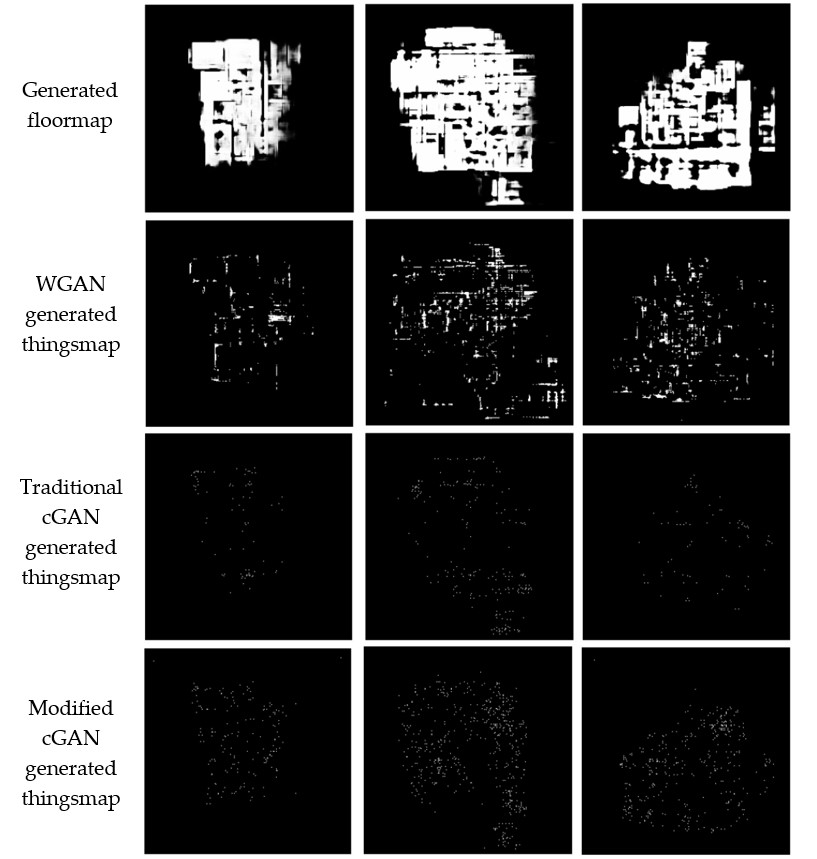
\includegraphics[width=1\textwidth]{sample_comparison.jpg}
    \caption[Generated things maps comparision]{ Generated things maps of the various models using levels generated by 
the WGAN-GP}
    \label{fig:samplecomparison}
\end{figure}

\chapter{Conclusion}
\label{ch:conclusion}%
The proposed system should serve as an early prototype for a more holistic format 
of procedural generating 3D levels using generative adversarial networks. The 
hybrid system has shown its prowess to suitably provide objects within a given level 
space and has solved any issues that could hinder gameplay from the previous 
design. It has proven its ability to provide the minimum subset of features needed 
to capture all the fundamental aspects of a level that can be exercised in isometric 
game engines by taking advantage of the simplicity of level structure in earlier 
games. This can be replicated in most games with a 2D map system to improve their 
replayability through the generation of multiple level layouts as well as multiple 
game object maps for each layout occasionally.

The models in this experiment are restrained to using the same dataset for the sake of 
maintaining consistency across all of the trained architectures. The system is open to 
improvement by modifying the dataset so that each model within the hybrid 
architecture can be fully utilized to its utmost potential. This can be done simply by 
altering the dataset that is used to train each of the models by tailoring it towards 
their strengths by means of reducing the image size and dropping the padding
entirely for the WGAN-GP subsystem while making use of this preprocessing for the 
cGAN with larger maps. This model can also incorporate other categories present within 
DOOM object types such as the obstacles and decorations.

While there are certain limitations and room for improvement, it stands as a better 
alternative to replaying levels in games, especially when they rely on ‘grinding’ 
the same maps to slow the pace at which the player progresses through its content 
to avoid them from finishing the game too quickly as it might indirectly affect their brand 
image. There is also the added benefit of reducing excessive dependence on content 
developers in designing every aspect of all the level and rather provide  intricate details 
to the ones that are cinematic in nature. This would maximize content in both quality and 
quantity by relying on such systems to provide generic levels as buffers between impactful 
set pieces and allow for an all around better pacing within games.

\section{Limitations}
There are a few constraints regarding its applicability to other games as it requires 
game data to be stored in a format where level structures can be easily decoded and 
parsed into image maps manually or through level builders with detailed 
specifications or guides. This system is also dependent on the game having a large 
collection of level instances created either by the studio or through effective tools for 
the community to build, access and share. Games are limited to simple terrains as it 
unable to represent multiple floors or stacked sections which are required to construct 
native 3D maps. It does not allow for different noisy images to consistently generate
significantly different category maps as there are usually very slight differences in 
their placements. There is also an issue in implementing doors and keys which need 
to be addressed as well as the use teleporters to connect detached segments within 
the level layout by including the respective triggers and landings in the generator 
before they can be used to incorporate concepts of puzzles within gameplay. 

\section{Future Works}
This system can be expanded by implementing additional models to separately learn 
the texture distribution of the level with the texture maps implemented through 
encoding pixels with texture id from a graphic dictionary and generated by 
means of a conditional network as used here. Conversely, by modifying the 
architecture to represent the textures map at lower resolutions, actual pixel colors can 
be encoded in the images to generate new graphics that are then extracted from the 
maps and encoded into their respective formats. Although this would  require image 
translation with super resolution models \cite{XuW22} that can generate the aesthetical features
together as the process would be dramatically upscaled for representing the
complete texture map at an acceptable resolution. 

By adding relations between pair of objects such as teleporters and landings or 
locked doors and keys that can be introduced through a separate feature map
representation, it can be used to improve the versatility of the generator to be used in
other genres as long as steps are taken to ensure that the levels generated meets the 
standard requirements such as solvability through additions made in the shortest 
path algorithms when considering these objects. The system can also be modified
with different sets of objects and used to train agents within simulated environments 
by learning a possible set actions or behaviors given certain objects present in them.


%-------------------------------------------------------------------------
%	BIBLIOGRAPHY
%-------------------------------------------------------------------------

\addtocontents{toc}{\vspace{2em}} % Add a gap in the Contents, for aesthetics
\bibliography{Thesis_bibliography} % The references information are stored in the file named "Thesis_bibliography.bib"

%-------------------------------------------------------------------------
%	APPENDICES
%-------------------------------------------------------------------------

\cleardoublepage
\addtocontents{toc}{\vspace{2em}} % Add a gap in the Contents, for aesthetics
\appendix
\chapter{Appendix A}
\label{appendixa}
\begin{large}
Ripley K Histograms
\end{large}
\begin{figure}[H]
    \centering
    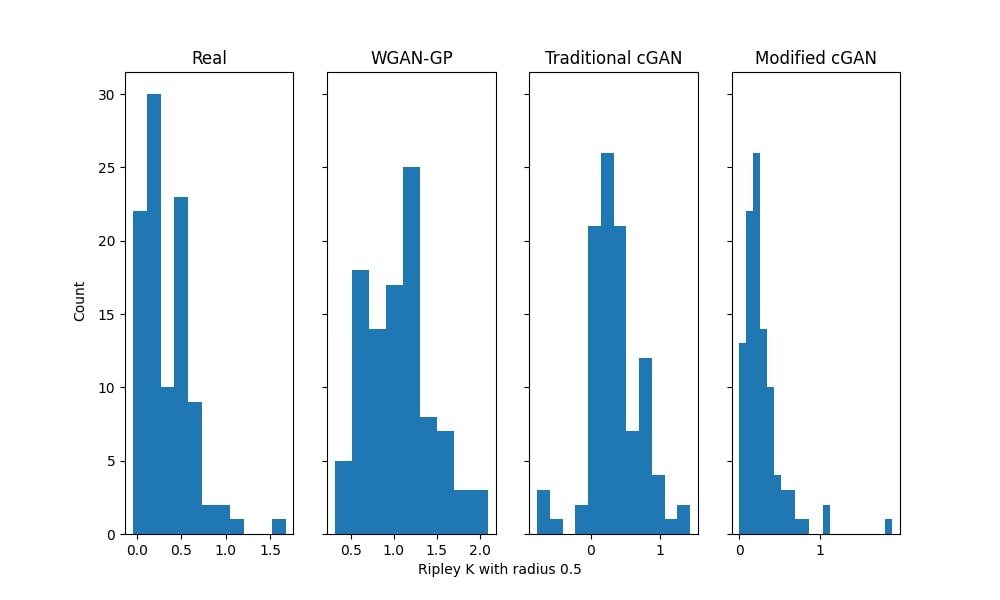
\includegraphics[width=0.9\textwidth]{ripk_5.jpg}
    \caption{Ripley K histogram with radius 0.5}
    \label{fig:ripk5}
\end{figure}
\begin{figure}[H]
    \centering
    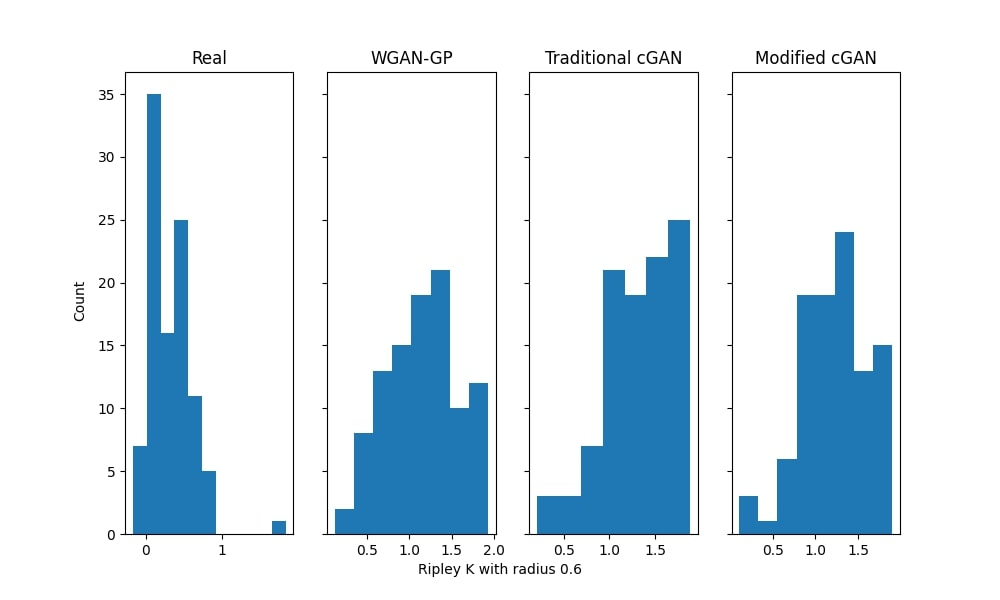
\includegraphics[width=0.9\textwidth]{ripk_6.jpg}
    \caption{Ripley K histogram with radius 0.6}
    \label{fig:ripk6}
\end{figure}
\begin{figure}[H]
    \centering
    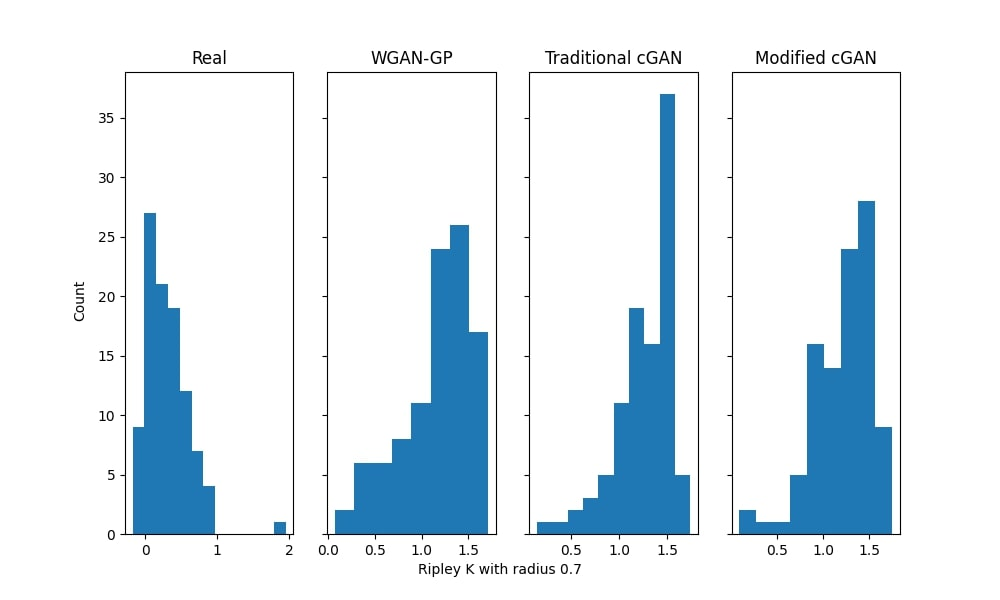
\includegraphics[width=0.9\textwidth]{ripk_7.jpg}
    \caption{Ripley K histogram with radius 0.7}
    \label{fig:ripk7}
\end{figure}
\begin{figure}[H]
    \centering
    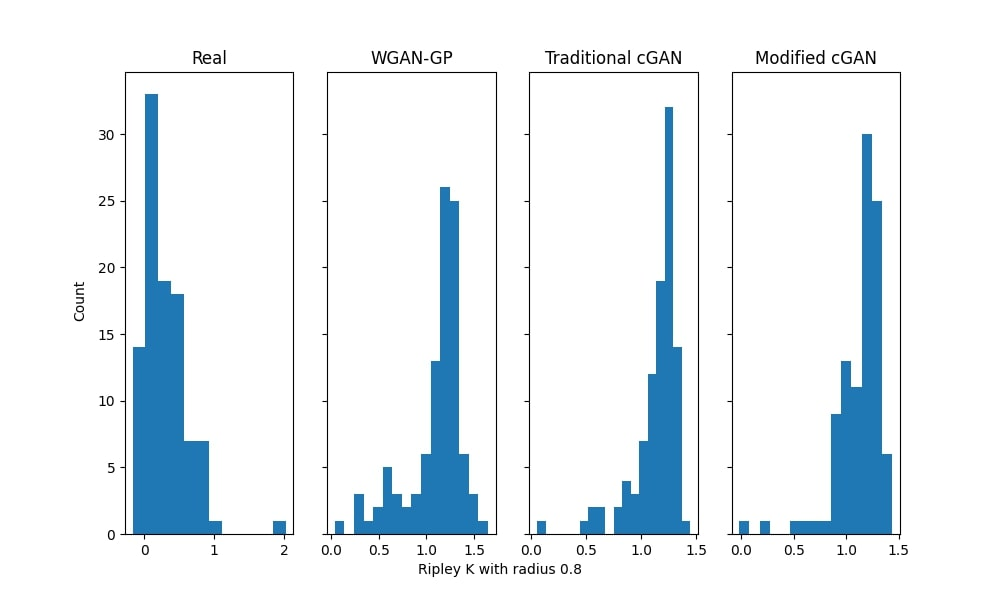
\includegraphics[width=0.9\textwidth]{ripk_8.jpg}
    \caption{Ripley K histogram with radius 0.8}
    \label{fig:ripk8}
\end{figure}
\begin{figure}[H]
    \centering
    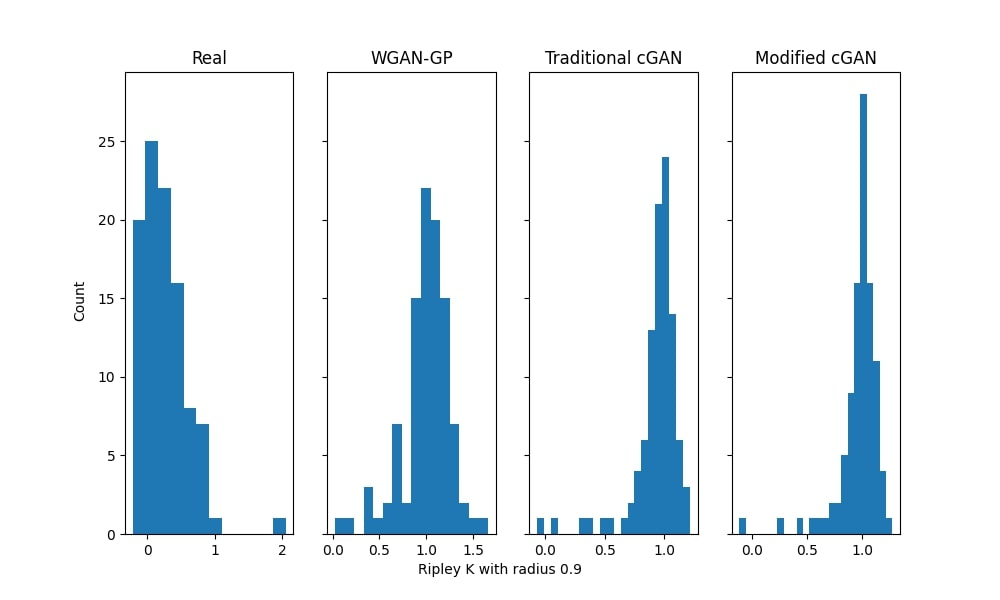
\includegraphics[width=0.9\textwidth]{ripk_9.jpg}
    \caption{Ripley K histogram with radius 0.9}
    \label{fig:ripk9}
\end{figure}
\begin{figure}[H]
    \centering
    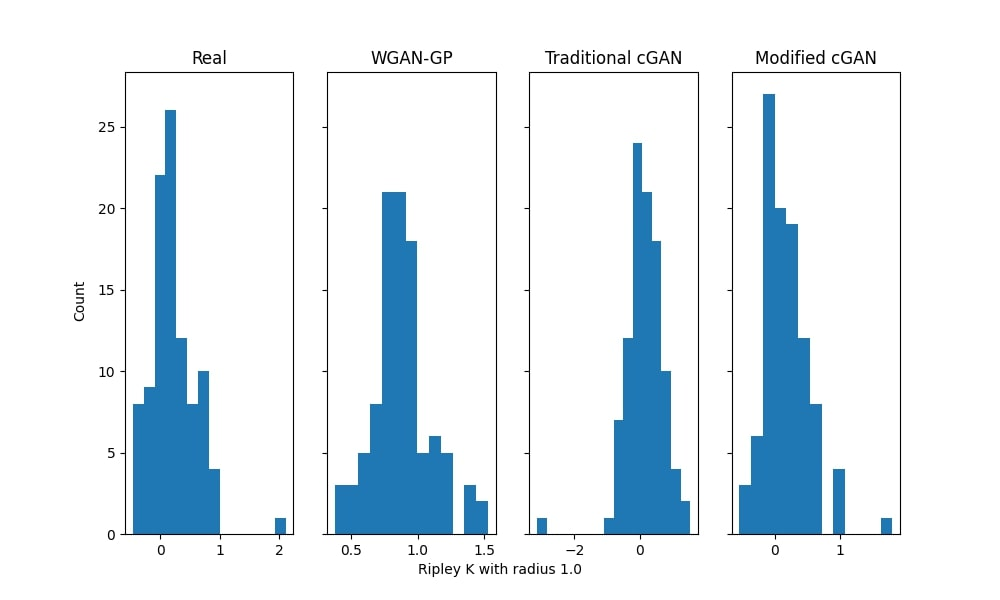
\includegraphics[width=0.9\textwidth]{ripk_10.jpg}
    \caption{Ripley K histogram with radius 1.0}
    \label{fig:ripk10}
\end{figure}

\chapter{Appendix B}
\label{appendixb}
\begin{large}
Game Objects Count by Type
\end{large}
\begin{figure}[H]
    \centering
    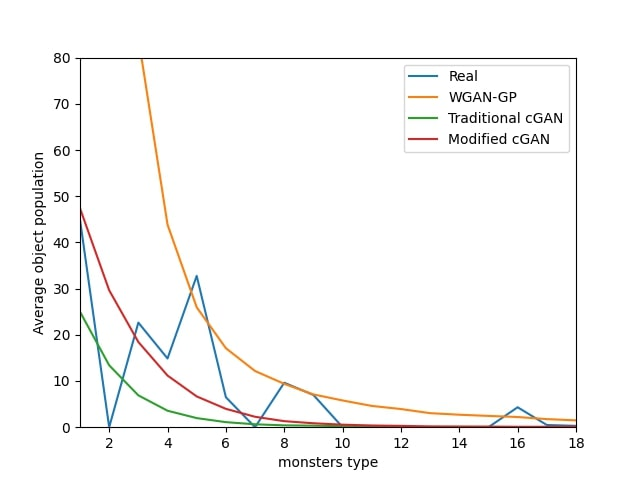
\includegraphics[width=0.8\textwidth]{monsters_count.jpg}
    \caption{Average monsters count by type in a level}
    \label{fig:monstercount}
\end{figure}
\begin{figure}[H]
    \centering
    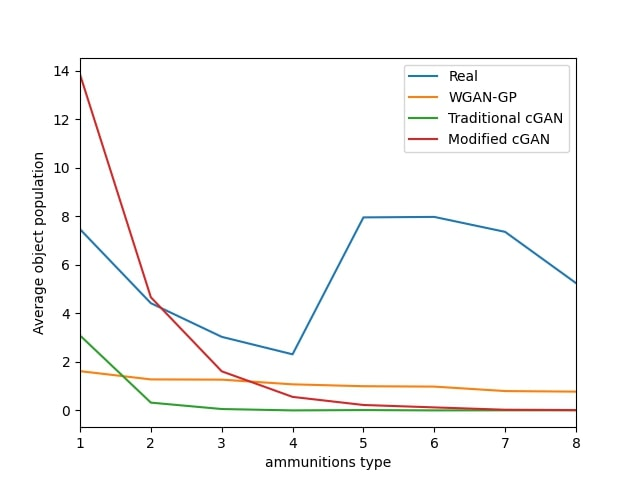
\includegraphics[width=0.8\textwidth]{ammunitions_count.jpg}
    \caption{Average ammunitions count by type in a level}
    \label{fig:ammunitionscount}
\end{figure}
\begin{figure}[H]
    \centering
    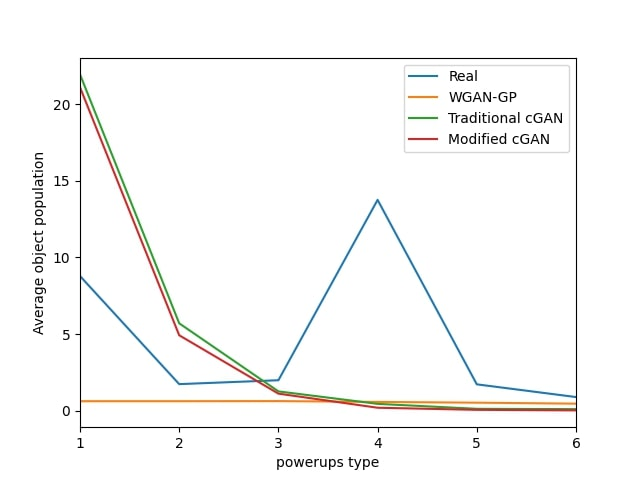
\includegraphics[width=0.8\textwidth]{powerups_count.jpg}
    \caption{Average powerups count by type in a level}
    \label{fig:powerupscount}
\end{figure}
\begin{figure}[H]
    \centering
    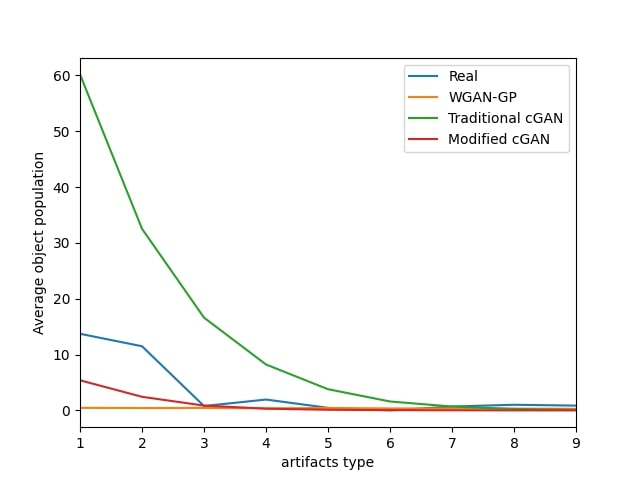
\includegraphics[width=0.8\textwidth]{artifacts_count.jpg}
    \caption{Average artifiacts count by type in a level}
    \label{fig:artifactscount}
\end{figure}
\begin{figure}[H]
    \centering
    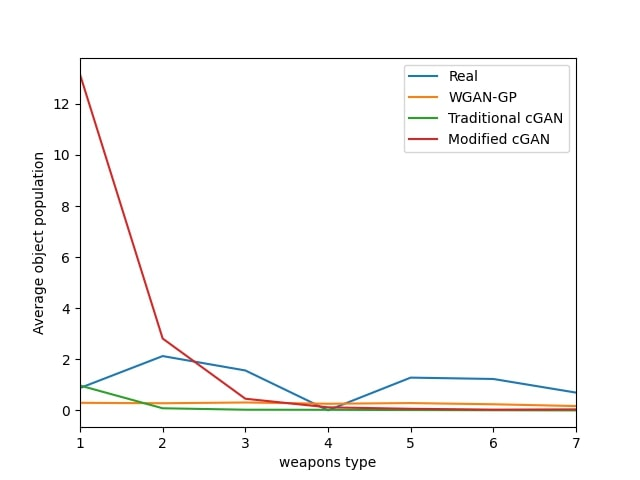
\includegraphics[width=0.8\textwidth]{weapons_count.jpg}
    \caption{Average weapons count by type in a level}
    \label{fig:weaponscount}
\end{figure}


% LIST OF FIGURES
\listoffigures

% LIST OF TABLES
\listoftables


% ACKNOWLEDGEMENTS
\chapter*{Acknowledgements}
I would like to thank my supervisor, Daniele Loiacono for the instructions he provided me that allowed me to write this thesis.
I thank my family and friends, especially my parents who supported me both financially and emotionally through this prolonged endeavor as well as provided me with their consistent encouragement which kept me motivated and stay on track towards completing this thesis. I express my gratitude towards Ali Emre Soleleyuk that sat through my venting during arising complications which let me have the breakthroughs that helped me progress towards its completion and Amrit A. with whom I was able to relax and redirect my focus towards actions that have been more productive.

\cleardoublepage

\end{document}
